% Chapters open on the next page rather than the next right-hand page:
% the template's double-sided openings leave a blank page before most
% chapters, which is right for binding and wrong for a PDF. No content
% is affected.
\PassOptionsToClass{openany}{book}
\documentclass{fast-nuces-bs}

\usepackage{mathptmx}% Times Roman font
\usepackage[T1]{fontenc}
\usepackage{sectsty}
\usepackage{titlesec}
\usepackage{booktabs}
\usepackage{longtable}
\usepackage{multirow}
\usepackage{array}
\usepackage{enumitem}
\usepackage{xcolor}
\usepackage{float}
\usepackage{caption}
\usepackage{tikz}
\usetikzlibrary{arrows.meta,positioning,shapes.geometric,calc,fit,backgrounds}
\usepackage{listings}
\usepackage{xurl}
\usepackage{adjustbox}

% Items the team must complete from their own records before submission are
% printed in red so none is missed.
\newcommand{\todo}[1]{\textcolor{red}{[#1]}}
\DeclareUrlCommand\code{\urlstyle{tt}}
\newcommand{\codex}[1]{\texttt{#1}}  % for captions and other moving arguments
\setlist{nosep}
\setlength{\emergencystretch}{2em}
\setlength{\tabcolsep}{4pt}
\lstset{basicstyle=\ttfamily\small,breaklines=true,frame=single,columns=fullflexible,keepspaces=true}

% Information about the project
% -----------------------------------------------------------------------------
\department{FAST School of Computing}
\faculty{Computer Science}
\degreeyear{2026}
\degreemonth{October}
\degreename{Computer Science}
\campuscity{Islamabad}
\authorone{Shahmir Khan Lughmani}{i220556}
\authortwo{Abbas}{i230803}
\authorthree{Abdullah Bin Nasir}{i230733}
\supervisor{Ms. Noshina Tariq}
\sessionduration{2023-2027}
\deanname{Dr. Dean Computing}
\directorname{Dr. Director of the Campus}
\hodname{Dr. Head of Computer Science Department}
\fypcoordinatorname{Name of FYP Coordinator}
\title{BlockLens: Launch-Risk Intelligence for Base Token Launches}
%%%%%%%%%%%%%%%%%%%%%%%%%%%%%%%%%%%%%%%%%%%%%%%%%%%%%%%%%%%%%%%%%%%%%%%%%%%%%%%

\begin{document}

\clearpage
\pagenumbering{roman}
\chapter*{Students' Submission}
\addcontentsline{toc}{chapter}{Students' Submission}
We certify that this report is submitted as the FYP-1 mid-report for the project titled

\begin{center}\textit{BlockLens: Launch-Risk Intelligence for Base Token Launches}\end{center}
\vspace{1cm}
\begin{tabular}{p{0.45\textwidth}p{0.45\textwidth}}
Student 1: Abdullah Bin Nasir & Signature: \rule{0.25\textwidth}{0.4pt}\\[1cm]
Student 2: Shahmir Khan Lughmani & Signature: \rule{0.25\textwidth}{0.4pt}\\[1cm]
Student 3: \todo{name, or delete} & Signature: \rule{0.25\textwidth}{0.4pt}
\end{tabular}

\chapter*{Anti-Plagiarism Statement}
\addcontentsline{toc}{chapter}{Anti-Plagiarism Statement}
The students certify that this report is their own work and that all sources used in preparing the report have been appropriately acknowledged and referenced. Every measurement quoted in this report was produced by the project's own code on the project's own data, and the script or report file that produced it is named where the number appears.

\chapter*{Authors' Declaration}
\addcontentsline{toc}{chapter}{Authors' Declaration}
We declare that the work documented in this report represents the work completed by the project team up to the FYP-1 mid-report stage. Contributions, tools, external components, and relevant sources are disclosed where applicable.

In particular, Section~\ref{sec:tools} discloses the use of an AI coding assistant during development. Every design decision, measurement and claim in this report was made, run and verified by the team; the assistant was used as a pair-programming and drafting tool under the team's direction, and its use is recorded in the repository's commit history.

\chapter*{Abstract}
\addcontentsline{toc}{chapter}{Abstract}
A new token pool is created on the Base blockchain roughly every minute, and most of the people who buy into one lose money: either the deployer withdraws the liquidity, or the price never recovers from its first hour. Existing tools either show market data without judgement, run static contract checks, or sell wallet labels behind a paid key. BlockLens reads the chain directly, judges every new launch once, at launch plus five minutes, and gives a trader two defended signals: who holds the liquidity (self-deployed and withdrawable, or launchpad and locked), and the probability that a buy at that moment is worth half or less six hours later.

The research half of the project built an ingestion and labelling pipeline on free, keyless sources; measured and corrected several published assumptions about those sources; defined outcome labels with a sensitivity analysis; found and removed label leakage and outcome censoring in an early model; and trained and validated the two signals on a properly sampled dataset of 1,066 launches in 841 operator families. The launch-type signal separates liquidity-pull rugs almost completely (109 of 113 self-deployed launches pulled against 0 of 74 launchpad launches); the buyer-loss model scores PR-AUC 0.83 in period and 0.76 out of time against 0.37 and 0.33 for a fixed rule checker. The wallet-graph features proposed as the project's central idea were found to add nothing on a properly powered test, and that negative result is reported rather than hidden.

The product half serves the signals live through a FastAPI service and a React front end: a Fresh Launches feed with push updates, an exact per-feature explanation of every score, a pre-registered forward record and paper-trading agent, a monitoring page for drift and outages, and a watchlist and history. A GitHub Actions pipeline type-checks, unit-tests, audits, end-to-end tests and builds both halves on every pull request, and publishes container images on every merge. The forward test, running since 19 October 2026, has resolved 850 predictions; the paper agent has passed its pre-registered floor and beats a buy-everything control by a margin of +55\% to +110\%. FYP-2 continues with a single investigation flow, an early-buyer screener over stored transfers, a retrained model on the forward record, and hosted deployment.

\chapter*{Acknowledgments}
\addcontentsline{toc}{chapter}{Acknowledgments}
The project team acknowledges the guidance and support received from the project supervisor, \todo{supervisor name}, the FYP committee of the FAST School of Computing, Islamabad, and the operators of the free public endpoints this project reads: the Tenderly public gateway for Base, DexScreener, GeckoTerminal and GoPlus. The project ran on their infrastructure as a polite guest and spent nothing.

\chapter*{Executive Summary}
\addcontentsline{toc}{chapter}{Executive Summary}

\textbf{The problem.} Base, an Ethereum layer-2 chain, sees thousands of new liquidity pools a day, of which around a hundred ever trade. Most of the tokens behind them lose their buyers' money within hours, either because the deployer withdraws the liquidity (a ``rug pull'') or because the price collapses from its launch spike. The information a buyer would need to avoid this exists on chain at the moment of launch, but no free tool reads it, judges it, and says how often its judgement has been right.

\textbf{The product.} BlockLens watches Base directly, discovers every new Uniswap V3 and V4 pool from the chain's own events, and judges each one once, at launch plus five minutes, with two signals the project's research can defend: the \emph{launch type} (self-deployed, so the deployer can withdraw liquidity; or launchpad, minted and locked in one transaction) and a \emph{buyer-loss risk} (the modelled probability that a buy at the minute-5 price is worth half or less at hour 6). Each score opens its own anatomy, an exact per-feature decomposition, and every prediction is written down before its outcome exists, so the product's accuracy is a public running score. Around the signal sit push updates, a paper-trading agent, a monitoring page, a watchlist and a history.

\textbf{What was found.} Several published assumptions about free data sources were wrong and were corrected by measurement. On this chain and population, liquidity-pull risk is decided almost entirely by launch type at minute 0. Buyer-loss risk inside the surviving population is predictable at PR-AUC 0.83 (0.76 out of time) against 0.37 for a fixed rule checker. The wallet-graph features that motivated the proposal add nothing over entry timing at either token or wallet level, on a properly powered test. An early model's apparently strong result was traced to label leakage and outcome censoring, withdrawn, and replaced by a redesigned dataset. The paper agent, run forward on 850 resolved launches, beats a buy-everything control by +55\% to +110\%; the page states that the edge comes from the launch-type filter rather than the risk score.

\textbf{Current state.} The core module is complete and live: ingestion, labels, sampling, two validated signals, a FastAPI service, the React front end, score explanations, push alerts, the paper agent's book, model health and persistence. A GitHub Actions pipeline runs 161 backend tests against PostgreSQL, 33 frontend unit tests, dependency audits and 7 browser end-to-end tests on every pull request, and publishes container images on every merge, scanned for vulnerabilities. Work flows through \code{main} $\leftarrow$ \code{develop} $\leftarrow$ \code{feature/*} with reviewed pull requests. The front end is deployed and open at \url{https://flying-boron-kxx29gy.tmp.now}, and the repository at \url{https://github.com/AbdullahBinNasir16/BlockLens} carries the current address.

\textbf{Scope decisions.} Features the research could not stand behind were cut rather than faked: KOL and social scoring (paid data only), a simulated portfolio, hand-authored wallet and narrative sections, and three unmeasured chains. The three hand-built project profiles remain as labelled case studies.

\textbf{Risks.} The forward test runs on one machine and has already suffered a 38-hour outage; hosting is the first FYP-2 task. The buyer-loss forward record is below its pre-registered floor for losses, so no accuracy claim is yet made on it. Free endpoints can change their limits without notice, as two already have.

\textbf{Remaining work.} FYP-2 delivers a single investigation flow for any Base address, an early-buyer wallet screener over stored transfers replacing the generated corpus, a model retrained on the forward record, and hosted deployment of the compose stack.

\chapter*{List of Abbreviations}
\addcontentsline{toc}{chapter}{List of Abbreviations}
\begin{tabular}{ll}
API & Application Programming Interface\\
AUC & Area Under the Curve\\
CI/CD & Continuous Integration / Continuous Delivery\\
CU & Compute Unit (a metered RPC request cost)\\
DEX & Decentralised Exchange\\
EOA & Externally Owned Account (a wallet)\\
ERC-20 & The Ethereum fungible token standard\\
FDV & Fully Diluted Valuation\\
FR & Functional Requirement\\
FYP & Final Year Project\\
GHCR & GitHub Container Registry\\
KOL & Key Opinion Leader (a promoting social account)\\
LP & Liquidity Pool / Liquidity Provider\\
NFR & Non-Functional Requirement\\
ORM & Object-Relational Mapper\\
PR & Pull Request\\
PR-AUC & Area under the Precision-Recall curve\\
ROC-AUC & Area under the Receiver Operating Characteristic curve\\
RPC & Remote Procedure Call (a blockchain node's JSON-RPC interface)\\
SHAP & SHapley Additive exPlanations\\
SSE & Server-Sent Events\\
UC & Use Case\\
V3, V4 & Uniswap protocol versions 3 and 4\\
WETH & Wrapped Ether\\
\end{tabular}


\clearpage
\pagenumbering{arabic}
\chapter{Introduction and Project Vision}

\section{Project Overview}
BlockLens is a launch-risk intelligence system for token launches on Base, an Ethereum layer-2 blockchain. It watches the chain directly, discovers every new Uniswap V3 and V4 liquidity pool from the chain's own events, and judges each launch once, at launch plus five minutes, with two signals: the \emph{launch type}, which says who can withdraw the pool's liquidity, and a \emph{buyer-loss risk}, the modelled probability that a purchase at that moment is worth half or less six hours later. The verdict, its exact anatomy, and a public running record of how often past verdicts were right are served by a FastAPI service to a React web application. Around the signal the product offers push alerts, a paper-trading agent that tests the signal forward, a monitoring page, a watchlist and an investigation history.

The system has two halves in one repository: a Python backend (\code{backend/}) that ingests, labels, samples, trains, scores live and serves; and a TypeScript front end (\code{src/}) that renders what the backend can defend and nothing it cannot. Both are built, tested and published by a GitHub Actions pipeline.

\section{Problem Statement}
On Base in 2026, Uniswap V4 alone emits about 3,100 pool-initialisation events a day, of which roughly 128 tokens a day are ever traded~\cite{decisions}. Of a random cohort of launches that were still alive five minutes after launch, 58\% had their liquidity pulled within ninety days, and among the launches that were not pulled, 93\% decayed to nothing. A retail buyer sees a new token on an aggregator minutes to hours after launch, with a price chart and no judgement. The facts that decide the outcome, in particular whether the deployer holds withdrawable liquidity, are readable on chain at minute zero, but no free tool reads them, states a verdict, explains it, and keeps score of its own accuracy.

The problem, stated as one sentence: \emph{given only what is observable on chain in a token's first five minutes, say how likely a buyer is to lose, say why, and prove it forward.}

\section{Problem Context and Motivation}
Three groups of people meet this problem. Retail traders, who buy new launches and carry the losses. Analysts and researchers, who want a reproducible, labelled record of what happened to launches and why. And platform operators, who need such a system to run unattended on free infrastructure and to report on itself.

The motivation is partly that the existing tools fall into three unsatisfying groups (Chapter~\ref{ch:research}): aggregators that show market data without judgement; static checkers that read contract code and miss the dominant failure mode on Base, which is behavioural rather than syntactic; and paid wallet-labelling services. It is also that the question is scientifically interesting: an earlier version of this project, and some of the literature, held that the structure of the wallet graph around a launch predicts its outcome. Measuring that claim properly, on a correctly sampled population with leakage and censoring controlled, was itself a contribution, and its answer (Section~\ref{sec:findings}) was not the expected one.

\section{Project Vision}
A trader opens BlockLens and sees every launch on Base judged within minutes of its birth, by a model whose validation record is printed beside every score, whose every verdict is logged before the outcome exists, and whose paper agent shows in public what the signal would have earned. Nothing on screen is invented; where a number is illustrative it says so.

\section{Project Objectives}
\begin{enumerate}[label=\textbf{O\arabic*}]
  \item Build an ingestion and labelling pipeline for Base on free, keyless sources, capable of a random cohort of at least 450 alive launches with outcome labels at 90 days. \emph{Achieved: 458 random-cohort tokens, 1,066 alive tokens in total.}
  \item Train and validate at least one launch-time signal that beats a pre-registered rule checker on a held-out, out-of-time set. \emph{Achieved: launch type, and buyer-loss PR-AUC 0.83 vs 0.37 in period, 0.76 vs 0.33 out of time.}
  \item Score every new Base launch live, within one minute of its five-minute mark, and serve it through an API with its validation record. \emph{Achieved; median scoring delay is reported on the Model Health page.}
  \item Keep a pre-registered forward record and report nothing below a floor of 200 resolved predictions with 20 losses. \emph{Running: 850 resolved, 14 losses as of 21 October 2026.}
  \item Explain every score exactly, as additive per-feature terms that sum to the model's own output. \emph{Achieved, asserted by a unit test to 1e-3.}
  \item Deliver both halves through a CI/CD pipeline with automated unit, API and end-to-end tests, protected branches and published artefacts. \emph{Achieved: 161 backend, 33 frontend and 7 end-to-end tests; images on GHCR.}
\end{enumerate}

\section{Project Scope}
\label{sec:scope}
The agreed scope is recorded in the repository as \code{docs/FYP1_SCOPE.md} and is summarised here.

\textbf{In scope, FYP-1 (core module).}
\begin{itemize}
  \item M1 Ingestion and labelling pipeline (Phases 1, 2, 5 of the decision log).
  \item M2 Launch risk signals: launch type and the buyer-loss model, with validation (Phases 5, 6).
  \item M3 Live scoring API and the Fresh Launches feed (Phase 7), with score explanations and push alerts (Phase 10).
  \item M4 Forward validation and the paper agent (Phases 8, 9), served as the Paper Agent page.
  \item M5 CI/CD and delivery: GitHub Actions for both halves, container images, production compose, branch process.
  \item M6 Token page for any Base contract: live market and security data merged with the BlockLens signal; watchlist and history; model health.
\end{itemize}

\textbf{In scope, FYP-2.} M7 one investigation flow; M8 richer persistence; M9 an early-buyer wallet screener over stored transfers, replacing the generated corpus; M10 a model retrained on the forward record; M11 hosting.

\textbf{Out of scope, and why.} KOL and social scoring need paid reads of X posts and there is no keyless substitute. A simulated portfolio was removed because invented trades beside a real record invite the question ``which of these is real''. Hand-authored wallet, narrative and social sections of the three case-study profiles were removed for the same reason. Chains other than Base are unmeasured. Accounts and multi-user state are deferred: the product is single-user by design at this stage.

\section{Project Modules}
\begin{table}[H]
\centering\small
\begin{tabular}{p{0.05\textwidth}p{0.3\textwidth}p{0.52\textwidth}}
\toprule
\# & Module & Responsibility\\
\midrule
M1 & Ingestion and labelling & Discover pools from chain events; backfill transfers and swaps in 1,000-block windows through a write gate that forbids lookahead; sample reserves and prices at historical blocks; assign RUG / FAILED / SURVIVED / NEVER\_LAUNCHED with a sensitivity analysis.\\
M2 & Signals & Case-control sampling with operator families; 23 token-level features at minute 5; launch-type rule; gradient-boosted buyer-loss model with calibration and out-of-time validation.\\
M3 & Live scoring and API & A scorer loop that discovers, waits for minute 5, backfills, scores, explains (tree SHAP) and alerts; FastAPI endpoints for the feed, token lookup, explanations, stream and health.\\
M4 & Forward record and paper agent & Append-only prediction log; outcomes resolved at hour 6 and days 1/7/30/90; pre-registered metrics and floors; four trading policies computed from the same rows.\\
M5 & Delivery & CI (typecheck, unit, API, audit, end-to-end), CD (GHCR images, release, scan, deploy hook), Dockerfiles, compose, branch protection, PR template.\\
M6 & Product surfaces & Fresh Launches, token page, Paper Agent, Model Health, Trending, Watchlist, History, three labelled case studies, a Sample-labelled wallet screener.\\
\bottomrule
\end{tabular}
\caption{Project modules and their responsibilities.}
\end{table}

\section{Stakeholders and User Classes}
\begin{itemize}
  \item \textbf{Retail trader.} Wants a verdict on a launch in seconds, a reason, and evidence the verdict is worth anything. Uses Fresh Launches, the token page, alerts and the watchlist.
  \item \textbf{Analyst or researcher.} Wants the labelled dataset, the model cards, the forward record and the decision log; reproducibility matters more than speed.
  \item \textbf{Operator.} Runs the stack; needs health, outages and drift visible, and a deployment that survives a reboot.
  \item \textbf{Supervisor and evaluators.} Need to see process: branches, reviews, tests, measured claims, honest negative results.
\end{itemize}

\section{Success Criteria}
\begin{enumerate}
  \item Every new Base Uniswap pool appears in the feed within one scan interval (60 s) and is scored or given a reason within one minute of its five-minute mark.
  \item Each signal's validation record is served with every score, and no score is shown without it.
  \item The forward record's success criteria, fixed on 19 October 2026 before any outcome, are met or the failure is reported: forward PR-AUC above the base rate with a bootstrap interval above zero, and a self-deployed 7-day pull rate above launchpad's.
  \item The paper agent's mean return beats the buy-everything control with the interval above zero. \emph{Met on 21 October 2026.}
  \item A pull request cannot merge into \code{develop} or \code{main} with a failing check.
\end{enumerate}

\section{Constraints and Assumptions}
\begin{itemize}
  \item \textbf{Unpaid work only.} No API key and no paid plan anywhere in the pipeline; the metered resource is politeness toward public endpoints, enforced by token buckets.
  \item \textbf{One chain.} Base runs at exactly 2.00 s per block (measured), so block numbers are the clock; every source, label and model is Base-specific.
  \item \textbf{Measured limits.} The keyless gateway caps \code{eth_getLogs} at 1,000 blocks and 20,000 results; archive \code{eth_call} works at least 365 days back; DexScreener allows 60 requests a minute.
  \item \textbf{Single user.} No accounts; product state has no owner column.
  \item \textbf{Development machine without Docker rights.} The store runs on a portable PostgreSQL in development; containers are built and tested in CI.
\end{itemize}

\section{Ethical, Legal and DEI Considerations}
\begin{itemize}
  \item \textbf{Pseudonymity.} The system groups addresses by behaviour and never attempts to identify a person; no column in any table can hold a name, handle, IP or KYC record, and the curated address lists name contracts, not people.
  \item \textbf{Not advice.} Every score is labelled as a model estimate about a launch at minute 5, not a recommendation; the paper agent moves no money and the page says so.
  \item \textbf{Honesty on screen.} Every section is marked Sourced or Sample; real projects never carry invented numbers; features that could only be faked were removed rather than shown.
  \item \textbf{Public infrastructure.} Rate limits are enforced client-side; the whole research phase cost the endpoint operators 297,000 requests spread over weeks, and no key was used.
  \item \textbf{Accessibility.} Body text is 16--17\,px, colour is never the only carrier of meaning (every tag also carries text), and \code{prefers-reduced-motion} disables all animation.
\end{itemize}

\chapter{Research and Existing Solutions}
\label{ch:research}

\section{Research Method / Approach}
The project treated every assumption about its data sources as a claim to be measured. Before any pipeline code was written, two sets of feasibility spikes (\code{backend/spikes/}, Parts A and B) probed each free endpoint for its real limits: request caps, block-range caps, archive depth, rate limits and the cost in calls of each operation the brief needed. Every number in the cost model is a measurement with the script that produced it. Decisions were written down as they were made, with their evidence, in \code{DECISIONS.md}; the file now runs to ten phases and records every deviation from the original brief, every bug that would have become a false finding, and every negative result.

Domain knowledge came from three places: the Uniswap V3 and V4 designs~\cite{uniswapv4}, which decide how pools, reserves and prices can be read; the academic literature on scam tokens and rug pulls on Ethereum DEXes~\cite{xia2021,mazorra2022,cernera2023}; and the evaluation literature for rare-event classification~\cite{saito2015,king2001,platt1999} and model explanation~\cite{lundberg2017,lundberg2020}.

\section{Concepts the System Rests On}
\label{sec:concepts}
The panel asked for evidence of understanding rather than description. These are the mechanisms the system is built on, each with the measurement that established how it behaves on Base.

\begin{description}
  \item[Pools, reserves and price.] A token launches when someone creates a liquidity pool pairing it with a quote asset (on Base, almost always WETH; of the first 2,064 swaps ingested, one was stablecoin-quoted). The pool holds a \emph{reserve} of each asset, and the price is their ratio (constant-product on V2-style pools, tick-based concentrated liquidity on V3 and V4, where \code{slot0} holds the current \code{sqrtPriceX96}). Prices in the store are kept as ratios against each token's own quote asset and used only to compare a token with its own peak, because a dollar price needs an ETH/USD series the project does not yet have.
  \item[Liquidity provider tokens and locks.] Whoever adds liquidity receives a claim on the pool (an LP token, or an NFT position on V3/V4) and can withdraw it. A ``rug pull'' in its dominant form is exactly that withdrawal: the token reserve collapses to zero in one transaction. \emph{Launchpad} factories (the 26 contracts in \code{known_addresses/launchpad.json}) mint the token and supply its liquidity in a single transaction and keep or burn the position, so the deployer has nothing to withdraw. Measured: 109 of 113 self-deployed launches in the held-out cohort were pulled; 0 of 74 launchpad launches were.
  \item[The three ways a launch loses its buyers' money.] Liquidity withdrawal (above); a supply dump, where early holders sell into later buyers (Phase 6 found this \emph{extraction} pattern in only 3.7\% of failed launches, against 93.1\% organic decay); and a honeypot, where the contract blocks selling (detected by simulation, which is GoPlus's job and not duplicated here).
  \item[Uniswap V4's singleton.] V3 deploys one contract per pool; V4 keeps every pool inside one \code{PoolManager} and identifies a pool by a 32-byte id. Three consequences were measured: V4 is about 95\% of Base launches (95 of 99 candidates in one window); a pool cannot be keyed by address, which broke two queries before tests caught them; and a per-pool quote reserve cannot be read from the singleton, which holds 4,211 WETH across all pools at once. The token side can be read exactly, because the singleton holds a given token only on account of that token's pools, and this was verified to the wei against stored transfers for five tokens.
  \item[Events, logs and topics.] Discovery and backfill read the chain's event logs: V4 \code{Initialize} and V3 \code{PoolCreated} for new pools, ERC-20 \code{Transfer} and the venue's \code{Swap} for activity. Topic hashes are computed with the project's own keccak and self-tested against the canonical \code{Transfer} topic rather than copied. Every free Base node caps \code{eth_getLogs} between 10 and 1,000 blocks (measured across six providers), which decides the whole cost model.
  \item[Archive state reads.] \code{eth_call} at a historical block returns the state as it was then. The free gateway answers at least 365 days back, so a reserve can be \emph{read} at 90 daily points in 43 s instead of \emph{reconstructed} from 3,888 log calls, and each reading is exact rather than a cumulative sum that one missed window would bias forever.
  \item[Blocks as the clock.] Base produces a block every 2.00 s exactly (measured over 43,200 blocks), so block numbers are timestamps: ``minute 5'' is block $b+150$, ``hour 6'' is $b+10{,}800$. Age is decided by block, never by an aggregator's timestamp, after one token arrived with a block from three days ago and a timestamp from 369 days ago.
  \item[Sniping, bundling and dispersers.] Bots buy in the launch block or within seconds (\code{t_same_block_buyers}, \code{t_first_buy_delay_s}); one address funding thousands of wallets across a handful of tokens is a disperser (airdrop or farm), which the graph module tells from infrastructure by wallets-per-token (1,080 for a disperser against 15 for the V4 \code{PoolManager}).
  \item[Lookahead.] A feature computed at minute 5 must only see rows from before minute 5. The write gate enforces this structurally (\code{as_of_ts} on every batch), and the Phase 5 audit showed what happens without it: a model that ``predicted'' rugs from a 24-hour window in which every rug had already happened.
\end{description}

\section{Existing Solutions / Products}
\label{sec:existing}
Each tool is described by what it reads and how it decides, from its public documentation and, where it is free, from using it. Two of them are wired into BlockLens itself.

\begin{description}
  \item[GoPlus Security (token security API).] Free, keyless, covers Base. Reads the token contract and its pools and returns structured flags: whether a sell is blocked (\emph{honeypot}, found by simulating a buy and a sell), buy and sell tax, whether the supply is mintable, whether ownership can be reclaimed or is hidden, whether the contract is a proxy or pausable, holder count, the top holders and their shares, and the LP holders with whether each position is locked. It is a \emph{static and simulation} check of the contract as it is now. BlockLens calls it for every token on the Trending and token pages (\code{fetchHolders}) and shows its holder count, top-10 share and honeypot flag with its name beside them. What it cannot do: judge the first five minutes of trading, say whether liquidity was \emph{minted and locked at launch} as a launch type, give a probability, or keep score of itself.
  \item[Token Sniffer (Solidus Labs).] A contract scanner that scores a token from an automated audit: known-scam code similarity, honeypot and fee checks, mint and ownership privileges, liquidity amount and lock status where it can read it. Strong on Ethereum and BSC; a score, not a probability; no forward record.
  \item[Honeypot checkers (honeypot.is and similar).] Simulate a buy and a sell against the live pool and report whether the sell succeeds and at what tax. A single question, answered well; BlockLens relies on GoPlus for the same question instead of re-implementing it.
  \item[RugCheck.] Solana-focused: mint and freeze authority, top-holder concentration, whether the LP is locked or burned. Not applicable to Base, but the ``is the LP locked'' idea is the same one launch type captures on Base.
  \item[DexScreener.] Indexes DEX pairs across chains and serves price, liquidity, volume, transactions, pair age and paid promotion status. No judgement. Measured: its ``new token'' and ``boosted'' feeds returned 60 rows with zero Base tokens, and it had indexed 20 of 99 launches that chain-event discovery found in the same window, so it is a display source, not a discovery source, for this chain. BlockLens uses it for symbols, liquidity and the pair table.
  \item[GeckoTerminal (CoinGecko).] Pool-level data and trending lists per network; BlockLens's Trending page reads its Base pool rankings. Metadata only.
  \item[Bubblemaps.] Draws holders as bubbles and groups wallets that transferred between each other, which shows concentration and insider clusters visually. Free for basic use on EVM chains. It is a \emph{picture} of the holder graph; BlockLens's Phase 3 built the same kind of graph and then measured, at full power, that its features add nothing to the two signals on this population, which is a result rather than a visualisation.
  \item[Nansen, Arkham.] Paid wallet labelling (``smart money'', exchange and fund attribution) and entity tracking. Closed data; the labels need an indexing API that no keyless source provides, which is why BlockLens's CEX list is empty by design rather than guessed.
  \item[DEXTools.] Pair charts and a listing score; paid tiers for the detail. No launch-time verdict.
  \item[Academic detectors.] Xia et al.~\cite{xia2021} characterised scam tokens on Uniswap V2 and trained a classifier on pool and trading features; Mazorra et al.~\cite{mazorra2022} detected rug pulls from token and liquidity features with gradient boosting; Cernera et al.~\cite{cernera2023} measured token spam, one-day rug pulls and sniper bots on Ethereum and BSC. All three are offline analyses of past launches; none runs live, explains a score, or logs predictions forward, and all predate V4's singleton.
\end{description}

\section{Comparison of Existing Solutions}
\label{sec:compare}
\begin{table}[H]
\centering\footnotesize
\setlength{\tabcolsep}{3pt}
\begin{tabular}{p{0.4\textwidth}cccccccc}
\toprule
Feature & \rotatebox{90}{GoPlus} & \rotatebox{90}{Token Sniffer} & \rotatebox{90}{DexScreener} & \rotatebox{90}{GeckoTerminal} & \rotatebox{90}{Bubblemaps} & \rotatebox{90}{Nansen / Arkham} & \rotatebox{90}{Academic} & \rotatebox{90}{\textbf{BlockLens}}\\
\midrule
Free, no API key & $\bullet$ & $\circ$ & $\bullet$ & $\bullet$ & $\circ$ & -- & n/a & $\bullet$\\
Covers Base, including Uniswap V4 pools & $\bullet$ & $\circ$ & $\bullet$ & $\bullet$ & $\circ$ & $\circ$ & -- & $\bullet$\\
Discovers launches from chain events (before aggregators) & -- & -- & -- & -- & -- & -- & $\circ$ & $\bullet$\\
Static contract checks (honeypot, tax, mint, owner) & $\bullet$ & $\bullet$ & $\circ$ & $\circ$ & -- & -- & $\circ$ & via GoPlus\\
Launch type: liquidity minted and locked at launch & $\circ$ & $\circ$ & -- & -- & -- & -- & -- & $\bullet$\\
Behavioural features of the first five minutes & -- & -- & -- & -- & -- & -- & $\circ$ & $\bullet$\\
A verdict at launch + 5 min, while a buyer can act & -- & -- & -- & -- & -- & -- & -- & $\bullet$\\
Probability from a model with published validation & -- & -- & -- & -- & -- & -- & $\bullet$ & $\bullet$\\
Exact per-score explanation & -- & $\circ$ & -- & -- & -- & -- & $\circ$ & $\bullet$\\
Pre-registered forward record of its own accuracy & -- & -- & -- & -- & -- & -- & -- & $\bullet$\\
Paper-trading test of the signal & -- & -- & -- & -- & -- & -- & -- & $\bullet$\\
Holder / wallet graph & $\circ$ & -- & -- & -- & $\bullet$ & $\bullet$ & $\bullet$ & $\circ$ (research only)\\
Push alerts & -- & -- & $\circ$ & -- & -- & $\bullet$ & -- & $\bullet$\\
Open method and code & -- & -- & -- & -- & -- & -- & $\bullet$ & $\bullet$\\
\bottomrule
\end{tabular}
\caption{Feature comparison. $\bullet$ provided; $\circ$ partial, or paid, or chain-limited; -- absent. Sources: each tool's public documentation and interface in October 2026; for GoPlus and DexScreener, their use inside BlockLens; for DexScreener's discovery, the measurement in \codex{backend/spikes/FINDINGS.md}.}
\label{tab:matrix}
\end{table}

Read down the BlockLens column, the product is not ``a better checker'': the static checks are deliberately delegated to GoPlus, which does them well. What no other tool in the table does is the middle block: watch the chain itself, judge the launch at the moment it can still be acted on from what the first five minutes show, and keep a public record of how right that judgement was.

\section{Limitations and Gaps}
Nothing free judges a Base launch at the moment it can still be acted on, says why, and keeps a public record of its own accuracy. The published detectors were trained on populations where rug and non-rug launches look structurally alike; on Base in 2026 the population is dominated by launchpad launches that mint and lock liquidity in one transaction, so their features and even their labels do not transfer unchanged. Two further gaps are practical: no keyless source exists for wallet funding provenance, and the public explorers that older write-ups treat as free fallbacks (Blockscout, Envio) now refuse keyless requests.

\section{Proposed Solution}
Read the chain, not the aggregators: discover pools from Uniswap's own events, backfill each pool's first minutes through a write gate that makes lookahead impossible, and sample reserves and prices at historical blocks with archive calls rather than reconstructing them from transfers. Define the outcome label explicitly, with every threshold a named constant and a sensitivity sweep over all of them. Sample properly: a random cohort at the true prevalence for every headline number, case-control strata for training, and operator families so no family crosses a split. Validate against pre-registered baselines and out of time. Then put the two signals that survive into a live service, explain each score exactly, log every prediction before its outcome, and run a paper agent on the record.

\section{Complex Computing Problem}
The project is a complex computing problem in the sense of the Washington Accord attributes:
\begin{itemize}
  \item \textbf{Conflicting requirements.} Completeness of data against the rule of unpaid work: the brief's method for labels (transfer reconstruction) cost 3,888 calls per token on the free gateway; the solution had to be re-derived (archive sampling, 90--232 calls) and shown to be more accurate, not less.
  \item \textbf{Depth of analysis.} The first model scored AUC 0.97 and was wrong: 64 of 85 features were downstream of the label, and all 28 labelled rugs had died inside their own feature window. Finding that required a leakage audit, a censoring analysis and a redesigned sampling frame.
  \item \textbf{No obvious solution.} Uniswap V4's singleton holds every pool's quote token in one contract, so the reserve a label needs cannot be read directly; the solution (read the \emph{token} side, which the singleton holds only on account of that token's pools) was derived and verified to the wei against stored transfers.
  \item \textbf{Infrequent and novel.} V4 is 95\% of Base launches and postdates the literature.
  \item \textbf{Beyond standard practice.} The product carries its validation record with every response, pre-registers its forward test and paper agent, and reports its own negative results.
\end{itemize}

\section{Contribution}
\label{sec:contribution}
What this project adds, each with the artefact that proves it:
\begin{enumerate}
  \item \textbf{A measured cost model for free Base data}, correcting four published assumptions (DexScreener discovery, Blockscout and Envio as keyless fallbacks, the log-range cap as an Alchemy quirk). \code{backend/spikes/FINDINGS.md}, \code{B_FINDINGS.md}.
  \item \textbf{Chain-event discovery and a lookahead-proof ingestion store}, resumable, budgeted, idempotent: 159 complete windows at 44 calls each, re-ingest byte-identical. \code{blocklens/ingest}, \code{store/write.py}, \code{test_write_gate.py}.
  \item \textbf{An explicit, swept outcome label} with a method for Uniswap V4's singleton (token-side reserve, verified to the wei). \code{label/rules.py}, \code{reports/label_sensitivity.md}.
  \item \textbf{A leakage and censoring audit} that withdrew the project's own first model, and a sampling design (random cohort, case-control strata, operator families) that fixed it. \code{reports/leakage_audit.md}, \code{reports/sampling_design.md}.
  \item \textbf{Two validated launch-time signals} on 1,066 launches: launch type (109/113 vs 0/74) and buyer-loss risk (PR-AUC 0.83 vs 0.37; 0.76 vs 0.33 out of time). \code{reports/model_card_v2.md}, \code{model_card_phase6.md}.
  \item \textbf{A negative result on wallet-graph features}, tested at full power at token and wallet level, reported rather than hidden. \code{model_card_v2.md} Part D.
  \item \textbf{A live scorer and API} that judges every new Base pool within a minute of its five-minute mark and serves every score with its validation record. \code{live/scorer.py}, \code{api/app.py}.
  \item \textbf{Exact score explanations} by tree SHAP on the frozen model, asserted additive by test. \code{live/explain.py}, \code{test_explain.py}.
  \item \textbf{A pre-registered forward test and paper agent}, protocol written before any outcome, with 850 resolved predictions and a passed floor. \code{live/resolver.py}, \code{reports/paper_agent.md}.
  \item \textbf{A delivery pipeline} with unit, API, audit and end-to-end tests on every pull request and scanned images on every merge. \code{.github/workflows/}.
\end{enumerate}

\section{Technical Challenges}
\begin{itemize}
  \item Every keyless Base RPC caps \code{eth_getLogs} between 10 and 1,000 blocks; Blockscout and Envio no longer serve keyless requests; DexScreener's feeds carry no Base launches.
  \item Uniswap V4 keys pools by id, not address, which broke two queries silently before they were caught (one would have produced a fabricated ``no co-movement'' finding).
  \item Label leakage through activity features, and outcome censoring: the median rug dies at minute 15, inside a 24-hour feature window.
  \item A regime shift: self-deployed launches went from 4--11\% to 63--69\% of the population in three months, which broke prior-shift calibration.
  \item No keyless source for ETH funding provenance, so graph edges are token-acquisition provenance, stated as such.
  \item A development machine without Docker rights, and a forward test that must survive reboots.
\end{itemize}

\section{Research Findings and Design Decisions}
\label{sec:findings}
\begin{table}[H]
\centering\small
\begin{tabular}{p{0.40\textwidth}p{0.47\textwidth}}
\toprule
Finding (measured) & Decision it drove\\
\midrule
DexScreener feeds: 0 Base tokens in 60 rows & Discovery reads chain events (V4 \code{Initialize}, V3 \code{PoolCreated})\\
Base = 2.00 s/block exactly & Block numbers are the clock; age by block, never by aggregator timestamp\\
1,000-block log cap; archive \code{eth_call} $\geq$ 365 d & Labels are sampled at blocks, not reconstructed; 90 points in 43 s\\
V4 singleton holds every quote reserve & Reserve criteria read the token side; verified exact to the wei on 5 tokens\\
64/85 features leak the label; all rugs die in-window & Phase 4 withdrawn; 5-minute window with survival requirement; family-grouped splits\\
20 RUG tokens formed one shared-wallet component & Operator families; cap 3 tokens per family; every CI resamples families\\
Launch type: 109/113 vs 0/74 & Launch type is a first-class signal, shown at minute 0\\
Graph features add +0.0003 at token level, AUC 0.52 at wallet level & Graph module kept as a documented negative result, not a product feature\\
FAILED splits 93\% decay / 4\% extraction & Buyer loss (price ratio at hour 6) is the product's second target\\
Buyer-loss PR-AUC 0.83 vs 0.37; 0.76 vs 0.33 out of time & Judged good enough to ship with its validation beside it\\
Self-deployed share shifted 4--11\% $\to$ 63--69\% & Model Health page tracks the drift; calibration reported before and after\\
Paper agent +49\% vs $-33\%$; LAUNCHPAD policy indistinguishable & The page states the edge is the launch-type filter\\
\bottomrule
\end{tabular}
\caption{Measured findings and the decisions they produced (details in \codex{DECISIONS.md}).}
\end{table}

\chapter{Proposal Feedback and Iteration Plan}

\section{Proposal Feedback Summary}
The proposal defence returned \emph{Approved with Minor Modifications} (project F26-090). The panel's comments, reproduced in full in Appendix~\ref{app:register}, make seven points: (1) the comparison with existing solutions must be in depth and feature by feature; (2) the team's own contribution must be made clear; (3) the comparison table showed no deep knowledge of existing systems or of blockchain concepts and read as copied from an LLM without proof; (4) the roadmap was not clear; (5) changes of scope must be addressed; (6) the team must work on the major tasks the system performs and understand how existing systems work; and (7) the system pipeline must be clearly defined: its components and how they interact.

Every point has been acted on, and the evidence for each is in this report and in the repository. The short version: the comparison is now built from using the tools and from measurement rather than description (Chapter~\ref{ch:research}); the contribution is enumerated with evidence (Section~\ref{sec:contribution}); the blockchain concepts the system rests on are set out and every number in the report reproduces from a named script (Section~\ref{sec:concepts}); the roadmap is a dated chart (Section~\ref{sec:roadmap}); the scope changes are recorded with reasons (Section~\ref{sec:scope} and \code{docs/FYP1_SCOPE.md}); the system runs live on its major tasks (Chapter~\ref{ch:iter1}); and the pipeline is drawn as components, interfaces and sequences (Chapter~\ref{ch:design}).

\section{Proposal Action Register}
\begin{longtable}{p{0.04\textwidth}p{0.27\textwidth}p{0.31\textwidth}p{0.08\textwidth}p{0.2\textwidth}}
\toprule
No. & Feedback / Required Change & Action Taken & Status & Evidence\\
\midrule
\endhead
1 & In-depth, feature-by-feature comparison with existing solutions & Nine tools and three papers reviewed by how they work, not by name; a 14-feature matrix; two of the tools (GoPlus, DexScreener) are integrated into BlockLens and used daily; DexScreener's discovery feeds were measured rather than assumed & Done & \S\ref{sec:existing}--\ref{sec:compare}; \code{src/lib/live/trending.ts}; \code{DECISIONS.md} 2026-10-11\\
2 & More work on the contribution part & Contributions enumerated with the artefact that proves each; per-member contribution with commit counts & Done & \S\ref{sec:contribution}; \S\ref{sec:contrib-members}\\
3 & No deep knowledge of existing systems and blockchain concepts; table copied from an LLM without proof & A concepts section written from the chain's own mechanics (pools, reserves, locks, V4's singleton, rug mechanisms) with the measurements that established each; every figure in the report names the script or report file that produced it & Done & \S\ref{sec:concepts}; \code{backend/spikes/FINDINGS.md}, \code{B_FINDINGS.md}\\
4 & Roadmap is not clear & Dated roadmap chart to the end of FYP-2 with modules, milestones and definition of done & Done & \S\ref{sec:roadmap}; Table~\ref{tab:fyp2}\\
5 & Address changes of scope & Scope fixed in a versioned document; every cut listed with its reason and its replacement; design evolution since the proposal stated & Done & \S\ref{sec:scope}; \S\ref{sec:evolution}; \code{docs/FYP1_SCOPE.md}\\
6 & Work on the major tasks the system performs; understand how existing systems work & The core module (ingest, label, score, serve, validate forward) is implemented and running live; existing tools described by mechanism & Done & Chapters~\ref{ch:iter1}, \ref{ch:test}; \S\ref{sec:existing}\\
7 & Define the pipeline: components and interactions & Architecture diagram, component table, API interface table, scorer sequence diagram, delivery pipeline, launch state diagram & Done & Figures~\ref{fig:arch}, \ref{fig:seq}, \ref{fig:cicd}; Table~\ref{tab:components}\\
\bottomrule
\end{longtable}

\section{Iteration Strategy}
Development is phase-gated and evidence-driven rather than time-boxed. Each phase states what it will measure before it runs, records its decisions and deviations in \code{DECISIONS.md} as they happen, and ends with a report in \code{backend/reports/} that a later phase can cite. Two practices from research methodology are applied to the product: \emph{pre-registration} (the forward test's metrics, floors and success criteria, and the paper agent's rules, were written down on 19 October 2026 before any outcome existed) and \emph{withdrawal} (the Phase 4 model card is marked withdrawn and its numbers may not be quoted).

On the engineering side the loop is the one in \code{CONTRIBUTING.md}: a feature branch from \code{develop}, small conventional commits, a pull request that CI must pass and a reviewer must approve, squash-merged; a release is a pull request from \code{develop} into \code{main} plus a version tag.

\section{Iteration 1 Plan}
\textbf{Dates:} 9 September to 19 October 2026. \textbf{Objective:} prove the data path and the signals, and build the interface the proposal showed.

\begin{itemize}
  \item \textbf{Selected features:} front-end prototype (profiles, screener, discovery pages); Phases 1--2 (ingestion, labels); Phase 3 (wallet graph); Phase 4 (first model) and its audit; Phase 5 (sampling, retrain, graph test); Phase 6 (buyer-loss target); Phase 7 (API, live feed).
  \item \textbf{Deliverables:} the labelled dataset and its data card; model cards v1 (withdrawn), v2 and Phase 6; the FastAPI service; the Fresh Launches page.
  \item \textbf{Evidence:} 24 commits, \code{backend/reports/*}, \code{DECISIONS.md} Phases 1--7.
\end{itemize}

\section{Iteration 2 Plan}
\textbf{Dates:} 19 to 22 October 2026 (continuing to the mid evaluation). \textbf{Objective:} prove the signal forward, deliver the product around it, and put both halves under CI/CD.

\begin{itemize}
  \item \textbf{Selected features:} Phase 8 forward validation; Phase 9 paper agent; Phase 10 score anatomy, push alerts, paper book, model health, watchlist and history; product cuts per scope; CI/CD pipeline; containers; end-to-end tests; this report.
  \item \textbf{Deliverables:} four pull requests (\#1--\#4), \code{docs/FYP1_SCOPE.md}, \code{CONTRIBUTING.md}, the report under \code{report/}.
  \item \textbf{Evidence:} CI runs on every pull request; \code{reports/paper_agent.md}; this document.
\end{itemize}

\section{Work Breakdown and Responsibilities}
\begin{table}[H]
\centering\small
\begin{tabular}{p{0.3\textwidth}p{0.3\textwidth}p{0.3\textwidth}}
\toprule
Area & Owner & Evidence\\
\midrule
Feasibility spikes, ingestion, labels, sampling, models, graph, live scorer, forward test & Abdullah Bin Nasir & commits 11--21 Oct; \code{backend/}; \code{DECISIONS.md}\\
Front-end prototype and design system & Abdullah Bin Nasir & commits 9--10 Sep; \code{src/}\\
CI/CD, containers, test strategy, unit and end-to-end tests, product rework, scope, report & Shahmir Khan Lughmani & commits 22 Oct; PRs \#1--\#4; \code{report/}\\
Score explanations, alerts, health, product state (API) & Shahmir Khan Lughmani (with Abdullah's review) & PR \#2\\
Proposal, presentations, tool survey, meeting records & Abbas & proposal document; Chapter~\ref{ch:research} sources; Appendix~F\\
\bottomrule
\end{tabular}
\caption{Work breakdown.}
\end{table}

\section{Progress Against Plan}
\begin{table}[H]
\centering\small
\begin{tabular}{p{0.34\textwidth}p{0.18\textwidth}p{0.18\textwidth}p{0.22\textwidth}}
\toprule
Milestone & Planned & Actual & Note\\
\midrule
Front-end prototype & Sep & 10 Sep & as proposed\\
Ingestion of 100 first-24h windows & Oct & 11 Oct (159) & target exceeded\\
Labelled set & Oct & 13 Oct (46) & then redesigned in Phase 5\\
Wallet graph and first model & Oct & 13 Oct & model withdrawn 18 Oct after audit\\
Powered dataset and retrain & -- & 18 Oct (1,066 alive) & added after the audit\\
Live API and feed & Oct & 19 Oct & \\
Forward test and paper agent & -- & 19 Oct, result 21 Oct & pre-registered\\
CI/CD pipeline & before mid-eval & 22 Oct & \\
Product rework and scope & before mid-eval & 22 Oct & \\
Mid report & before mid-eval & 22 Oct (draft) & this document\\
\bottomrule
\end{tabular}
\caption{Planned milestones against actual progress.}
\end{table}

\section{Delays, Deviations and Recovery Plan}
\begin{itemize}
  \item \textbf{The first model was wrong, and was withdrawn.} Phase 4 reported AUC 0.79/0.97 from entry timing. The Phase 5 audit showed total outcome censoring and label leakage. Recovery: a 5-minute feature window with a survival requirement, a random cohort, case-control training strata and operator families; the retrain produced the two signals the product ships. Cost: about four days; benefit: every number now survives an adversarial reading.
  \item \textbf{A 38-hour outage of the forward test} (19--21 October) after a machine restart. Recovery: an auto-start task; a rule, set before any late row was scored, that only timely predictions count; late-due launches logged as missed rather than scored. Hosting the stack on a server is FYP-2's first task.
  \item \textbf{Keyless sources moved.} Blockscout and Envio stopped serving keyless requests; DexScreener's feeds proved useless for Base discovery. Recovery: chain-event discovery, archive sampling, GoPlus for holder data.
  \item \textbf{Scope was wider than the research could support.} Recovery: the scope document and the product cuts of Phase 10, recorded with reasons, so the panel sees a product that is narrower and entirely real rather than wider and half sample.
\end{itemize}

\chapter{Software Requirements}
\label{ch:req}

\section{User Interactions / Use Cases}
\begin{table}[H]
\centering\small
\begin{tabular}{p{0.07\textwidth}p{0.25\textwidth}p{0.17\textwidth}p{0.41\textwidth}}
\toprule
ID & Use case & Actor & Goal\\
\midrule
UC1 & Watch fresh launches & Trader & See every new Base pool judged at minute 5, with status or reason, updating live\\
UC2 & Read a score's anatomy & Trader, Analyst & See which observations moved a score and which way\\
UC3 & Investigate an address & Trader & Paste any Base contract and get live data plus the BlockLens signal if tracked\\
UC4 & Receive an alert & Trader & Be told, in the page or by Telegram, when a launch the agent would buy is scored\\
UC5 & Keep a watchlist & Trader & Star tokens and find them again\\
UC6 & Review history & Trader & Reopen past investigations\\
UC7 & Read the forward record & Analyst, Evaluator & See the paper agent's book and the pre-registered metrics\\
UC8 & Monitor the system & Operator & See scan status, volume by reason, drift, calibration and outages\\
UC9 & Browse trending tokens & Trader & Discovery over live Base pools\\
UC10 & Deliver a change & Developer & Open a PR, pass CI, merge, publish images\\
\bottomrule
\end{tabular}
\caption{Use cases.}
\end{table}

\section{Use Case Diagram}
\begin{figure}[H]
\centering
\begin{adjustbox}{max width=\textwidth}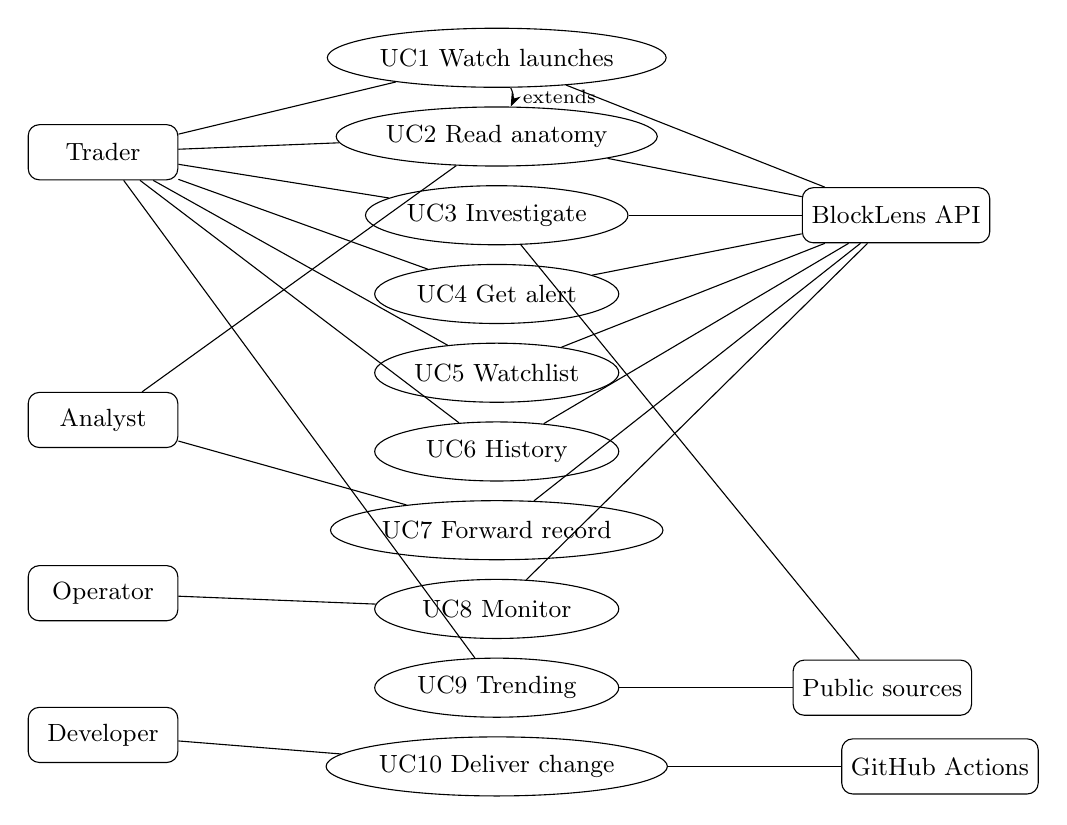
\begin{tikzpicture}[font=\small, actor/.style={draw, rounded corners, minimum width=1.9cm, minimum height=0.7cm}, uc/.style={draw, ellipse, minimum width=3.1cm, minimum height=0.75cm, align=center, inner sep=1pt}, node distance=0.35cm]
  \node[actor] (trader) at (0,0) {Trader};
  \node[actor] (analyst) at (0,-3.4) {Analyst};
  \node[actor] (op) at (0,-5.6) {Operator};
  \node[actor] (dev) at (0,-7.4) {Developer};
  \node[uc] (uc1) at (5,1.2) {UC1 Watch launches};
  \node[uc] (uc2) at (5,0.2) {UC2 Read anatomy};
  \node[uc] (uc3) at (5,-0.8) {UC3 Investigate};
  \node[uc] (uc4) at (5,-1.8) {UC4 Get alert};
  \node[uc] (uc5) at (5,-2.8) {UC5 Watchlist};
  \node[uc] (uc6) at (5,-3.8) {UC6 History};
  \node[uc] (uc7) at (5,-4.8) {UC7 Forward record};
  \node[uc] (uc8) at (5,-5.8) {UC8 Monitor};
  \node[uc] (uc9) at (5,-6.8) {UC9 Trending};
  \node[uc] (uc10) at (5,-7.8) {UC10 Deliver change};
  \node[actor, right=2.2cm of uc3] (api) {BlockLens API};
  \node[actor, right=2.2cm of uc9] (src) {Public sources};
  \node[actor, right=2.2cm of uc10] (gh) {GitHub Actions};
  \foreach \u in {uc1,uc2,uc3,uc4,uc5,uc6,uc9} \draw (trader) -- (\u);
  \foreach \u in {uc2,uc7} \draw (analyst) -- (\u);
  \draw (op) -- (uc8);
  \draw (dev) -- (uc10);
  \foreach \u in {uc1,uc2,uc3,uc4,uc5,uc6,uc7,uc8} \draw (\u) -- (api);
  \foreach \u in {uc3,uc9} \draw (\u) -- (src);
  \draw (uc10) -- (gh);
  \draw[dashed,-{Stealth}] (uc1) to[bend left=25] node[right,font=\scriptsize]{extends} (uc2);
\end{tikzpicture}\end{adjustbox}
\caption{Use case diagram.}
\end{figure}

\section{Detailed Use Cases}
\begin{table}[H]
\centering\small
\begin{tabular}{p{0.2\textwidth}p{0.70\textwidth}}
\toprule
\multicolumn{2}{l}{\textbf{UC3 Investigate an address}}\\
\midrule
Actor & Trader\\
Precondition & The web app is open; the API is reachable (for the signal) or not (live data still shows)\\
Main flow & 1. The user pastes a contract address on New Investigation and presses Investigate. 2. If the address is one of the three case studies, the research animation plays and the profile opens. 3. Otherwise the token page opens: DexScreener market data, GoPlus holders and flags, the pools. 4. The API is asked whether the launch was tracked; if so, launch type, risk and the score's anatomy are shown. 5. The visit is recorded in history.\\
Alternative & 3a. Not an address: the field says so and nothing is submitted. 3b. A source is unreachable: that section shows an error, the others still load. 4a. The API is down: the page says the signal is unavailable; the Watch button is disabled.\\
Postcondition & A history row exists; no sample section was shown under the real token's name\\
\midrule
\multicolumn{2}{l}{\textbf{UC1 Watch fresh launches}}\\
\midrule
Actor & Trader\\
Precondition & The API is running with its live loop\\
Main flow & 1. Fresh Launches loads the feed and the model's validation record. 2. The page polls every 30 s and subscribes to the push stream. 3. A pool appears as ``waiting for minute 5''; at its five-minute mark it is scored or given a reason. 4. A newly scored launch arrives by push as a toast; if permitted and the agent would buy it, a browser notification fires. 5. The user opens the why-button for the anatomy or the row for the token page.\\
Alternative & 2a. The stream drops: the status says ``Push off'' and polling continues. 3a. The scorer cannot read the chain: the pool shows ``could not read the first 5 minutes''.\\
Postcondition & Every scored launch is logged once in the forward record\\
\midrule
\multicolumn{2}{l}{\textbf{UC10 Deliver a change}}\\
\midrule
Actor & Developer\\
Main flow & 1. Branch from \code{develop}. 2. Commit; push; open a PR with the template. 3. CI runs: typecheck, unit tests with a coverage floor, build; backend tests on PostgreSQL; audits; end-to-end. 4. A reviewer approves. 5. Squash-merge; CD publishes the \code{develop} image tag. 6. A PR from \code{develop} to \code{main} and a tag publish \code{latest}, a release, and trigger the deploy hook.\\
Alternative & 3a. A check fails: the merge button is blocked until it is green.\\
\bottomrule
\end{tabular}
\caption{Detailed use cases (the remainder are in Appendix~\ref{app:req}).}
\end{table}

\section{Functional Requirements}
\subsection{M1 Ingestion and labelling}
\begin{itemize}[label={}]
  \item \textbf{FR-1.1} The system shall discover new pools from Uniswap V4 \code{Initialize} and V3 \code{PoolCreated} events, polling at a configurable interval.
  \item \textbf{FR-1.2} The system shall backfill each pool's transfers and swaps in 1,000-block windows, resumable from a checkpoint.
  \item \textbf{FR-1.3} Every row shall enter the store through one write gate that takes an explicit \code{as_of_ts} and rejects any batch containing a later timestamp.
  \item \textbf{FR-1.4} Every metered call shall pass through a token bucket per source and a per-run ceiling.
  \item \textbf{FR-1.5} The system shall sample each token's reserve and price at historical blocks and assign RUG, FAILED, SURVIVED or NEVER\_LAUNCHED by named criteria, storing the observations with the verdict.
  \item \textbf{FR-1.6} A sensitivity sweep shall re-derive every verdict offline at any threshold.
\end{itemize}
\subsection{M2 Signals}
\begin{itemize}[label={}]
  \item \textbf{FR-2.1} Training shall use a random cohort at true prevalence for evaluation and case-control strata for fitting, grouped by operator family, with no family crossing a split.
  \item \textbf{FR-2.2} The launch-type signal shall be read at minute 0 from whether the token was minted and supplied with liquidity in one transaction.
  \item \textbf{FR-2.3} The buyer-loss model shall be scored once, at minute 5, only for pools that traded by then and still hold their liquidity.
  \item \textbf{FR-2.4} Every model shall be compared against a pre-registered rule checker, in period and out of time, and shipped with that record.
\end{itemize}
\subsection{M3 Live scoring and API}
\begin{itemize}[label={}]
  \item \textbf{FR-3.1} The scorer shall find new pools every 60 s and score each at its five-minute mark, or record the reason it was not scored.
  \item \textbf{FR-3.2} Every API response carrying a score shall carry the model's validation record.
  \item \textbf{FR-3.3} Every score shall carry its anatomy: per-feature log-odds terms that sum to the score, with labels and display values.
  \item \textbf{FR-3.4} The API shall push newly scored launches over server-sent events and, when configured, to Telegram for launches matching the paper agent's buy rule.
  \item \textbf{FR-3.5} \code{GET /api/token/{address}} shall return the launch's signals if tracked and say so if not; a non-address is rejected with 400.
\end{itemize}
\subsection{M4 Forward record and paper agent}
\begin{itemize}[label={}]
  \item \textbf{FR-4.1} Every prediction shall be written once, at scoring time, and never edited; unscored launches are logged with their reason.
  \item \textbf{FR-4.2} Buyer loss shall be resolved at hour 6 by the same code as the label; liquidity at days 1, 7, 30 and 90.
  \item \textbf{FR-4.3} No forward metric shall be called a result below 200 resolved predictions with 20 losses; the paper agent needs 100 trades.
  \item \textbf{FR-4.4} Only predictions scored before their outcome existed shall count; late ones are counted separately.
  \item \textbf{FR-4.5} The API shall serve the book trade by trade, and the pages shall derive every performance figure from those rows.
\end{itemize}
\subsection{M5 Delivery}
\begin{itemize}[label={}]
  \item \textbf{FR-5.1} Every push and pull request shall run typecheck, unit tests with a coverage floor, build, backend tests on PostgreSQL, dependency audits and end-to-end tests.
  \item \textbf{FR-5.2} A merge to \code{develop} or \code{main} shall publish container images for both halves, tagged by branch, sha and semver, and scan them.
  \item \textbf{FR-5.3} A version tag shall create a GitHub Release with the web bundle attached.
  \item \textbf{FR-5.4} \code{main} and \code{develop} shall require a pull request, one approval and green checks.
\end{itemize}
\subsection{M6 Product surfaces}
\begin{itemize}[label={}]
  \item \textbf{FR-6.1} Fresh Launches shall show every tracked pool with status, launch type, risk, minute-5 counts, a why-button, push toasts and an optional browser notification.
  \item \textbf{FR-6.2} The token page shall never show a sample section under a real token's name.
  \item \textbf{FR-6.3} The user shall be able to star any token or case study and see the watchlist; every investigation shall be recorded in history.
  \item \textbf{FR-6.4} Model Health shall show scan status, launches a day by reason, launch-type drift, forward calibration and outages.
  \item \textbf{FR-6.5} Every section with illustrative data shall carry a Sample chip.
\end{itemize}

\section{Non-Functional Requirements}
\subsection{Reliability}
NFR-R1 The scorer loop shall survive any failing tick and report the error on \code{/api/health}. NFR-R2 A crashed backfill shall resume from its checkpoint; re-ingesting a token shall leave the store byte-identical (verified). NFR-R3 A failed alert shall never stop scoring. NFR-R4 An outage shall cost coverage, never correctness: late-due launches are logged as missed.
\subsection{Usability}
NFR-U1 Body text 16--17\,px, colour never the sole carrier of meaning. NFR-U2 Every number says where it came from (Sourced / Sample / live API). NFR-U3 Empty and error states name the cause and a next step. NFR-U4 Works at phone width; the sidebar becomes a drawer below 900\,px.
\subsection{Performance}
NFR-P1 A launch is scored within 60 s of its five-minute mark under normal load (median delay shown on Model Health). NFR-P2 The production bundle is under 100\,KB gzipped of application code (currently 79\,KB). NFR-P3 No chart library; geometry computed once; scroll work rAF-throttled. NFR-P4 The screener evaluates 400 wallets in under 1\,ms.
\subsection{Security}
NFR-S1 No API key or secret in the repository; alert credentials only from the environment. NFR-S2 The test suite blocks the network transport so no test can leak a call. NFR-S3 Dependencies audited on every PR; images scanned on every publish. NFR-S4 Input addresses validated server-side; product state has no path to code execution. NFR-S5 The write gate makes lookahead structurally impossible.

\section{Acceptance Criteria}
\begin{table}[H]
\centering\small
\begin{tabular}{p{0.12\textwidth}p{0.47\textwidth}p{0.32\textwidth}}
\toprule
Req. & Check & Status\\
\midrule
FR-1.3 & A batch with one row after \code{as_of_ts} raises \code{LookaheadError} and writes nothing & pass (\code{test_write_gate.py})\\
FR-1.5 & Labels re-derived from stored series at every threshold; 90-day baseline reclassifies 0\%, 30-day 10.9\% & pass (\code{label_sensitivity.md})\\
FR-2.4 & PR-AUC 0.83 vs 0.37 in period; 0.76 vs 0.33 out of time & pass (\code{model_card_phase6.md})\\
FR-3.2 & Every \code{/api/launches} response carries \code{model.validation} & pass (\code{test_api.py})\\
FR-3.3 & Anatomy terms sum to the model's logit within 1e-3 & pass (\code{test_explain.py})\\
FR-4.3 & Pages show ``too early'' below the floor & pass (visible on Fresh Launches)\\
FR-5.1 & CI run on PR \#4 shows all jobs & pass\\
FR-5.4 & Branch protection on \code{main}, \code{develop} & not available: GitHub offers protection rules on a private repository only on a paid plan, or on a public one. Enforced by convention instead (every change on \code{develop} is a reviewed, CI-green pull request, as the merge history shows); it is switched on the day the repository is made public\\
FR-6.3 & Watchlist round trip via API in the browser & pass (\code{e2e/smoke.spec.ts})\\
\bottomrule
\end{tabular}
\caption{Acceptance checks for the important requirements.}
\end{table}

\section{Requirements Traceability}
\begin{table}[H]
\centering\small
\begin{tabular}{p{0.1\textwidth}p{0.08\textwidth}p{0.3\textwidth}p{0.40\textwidth}}
\toprule
Req. & Module & Implementation & Tests\\
\midrule
FR-1.1--1.2 & M1 & \code{ingest/chain.py}, \code{ingest/runner.py} & \code{test_decode.py}, \code{test_sources.py}\\
FR-1.3 & M1 & \code{store/write.py} & \code{test_write_gate.py}\\
FR-1.4 & M1 & \code{ingest/budget.py} & \code{test_budget.py}\\
FR-1.5--1.6 & M1 & \code{label/rules.py}, \code{label/sample.py}, \code{scripts/label_sensitivity.py} & \code{test_label_rules.py}, \code{test_label_fixtures.py}, \code{test_reserve_method.py}\\
FR-2.1 & M2 & \code{sampling/design.py} & \code{test_phase5.py}\\
FR-2.2--2.4 & M2 & \code{model/token_features.py}, \code{scripts/phase5_model.py}, \code{phase6_model.py}, \code{rulecheck_x.py} & \code{test_model.py}\\
FR-3.1--3.2 & M3 & \code{live/scorer.py}, \code{api/app.py} & \code{test_api.py}\\
FR-3.3 & M3 & \code{live/explain.py} & \code{test_explain.py}\\
FR-3.4 & M3 & \code{live/alerts.py}, \code{/api/stream} & \code{test_alerts.py}, \code{test_product_api.py}\\
FR-4.1--4.5 & M4 & \code{live/resolver.py} & \code{test_product_api.py}; forward checks vs 4 research tokens\\
FR-5.1--5.3 & M5 & \code{.github/workflows/ci.yml}, \code{cd.yml} & the runs themselves\\
FR-6.1 & M6 & \code{routes/Launches.tsx}, \code{components/live/Explain.tsx} & \code{launches.test.ts}, \code{e2e}\\
FR-6.3 & M6 & \code{lib/live/product.ts}, \code{WatchlistPage.tsx} & \code{e2e}\\
FR-6.4 & M6 & \code{routes/ModelHealth.tsx}, \code{lib/live/health.ts} & \code{health.test.ts}, \code{e2e}\\
\bottomrule
\end{tabular}
\caption{Traceability from requirements to modules, code and tests.}
\end{table}

\chapter{System Design}
\label{ch:design}

\section{System Architecture}
\begin{figure}[H]
\centering
\begin{adjustbox}{max width=\textwidth}\begin{tikzpicture}[font=\small, box/.style={draw, rounded corners, align=center, minimum height=0.9cm, inner sep=5pt}, ext/.style={box, dashed}, >={Stealth}]
  % external sources
  \node[ext] (rpc) at (0,6) {Base RPC\\(Tenderly public gateway)};
  \node[ext] (ds) at (4.6,6) {DexScreener};
  \node[ext] (gt) at (8.2,6) {GeckoTerminal\\GoPlus};
  \node[ext] (tg) at (12,6) {Telegram Bot API};
  % backend
  \node[box, minimum width=3.6cm] (ingest) at (0,3.6) {Ingest\\discover, backfill,\\budget, write gate};
  \node[box, minimum width=3.4cm] (label) at (4.1,3.6) {Label \& sample\\rules, archive reads,\\families};
  \node[box, minimum width=3.2cm] (model) at (8,3.6) {Model\\features, training,\\\code{buyer_loss_v1}};
  \node[box, minimum width=3.6cm] (live) at (12,3.6) {Live\\scorer, explain,\\resolver, alerts};
  \node[box, minimum width=5.2cm] (db) at (2.6,1.2) {PostgreSQL 16 (+TimescaleDB)\\16 tables, Alembic migrations};
  \node[box, minimum width=5.2cm] (api) at (9.6,1.2) {FastAPI service\\feed, token, explain, stream,\\paper book, health, watchlist, history};
  % frontend
  \node[box, minimum width=11cm] (web) at (6,-1.3) {React + TypeScript web app (Vite)\\Fresh Launches, token page, Paper Agent, Model Health, Trending, Watchlist, History, case studies};
  \node[box, minimum width=11cm] (ci) at (6,-3.2) {GitHub Actions: CI (typecheck, unit, API, audit, e2e) $\cdot$ CD (GHCR images, release, Trivy, deploy hook)};
  \draw[->] (rpc) -- (ingest);
  \draw[->] (rpc) -- (label);
  \draw[->] (rpc) -- (live);
  \draw[->] (ds) -- (ingest);
  \draw[->] (ingest) -- (db);
  \draw[->] (label) -- (db);
  \draw[<->] (model) -- (db);
  \draw[<->] (live) -- (db);
  \draw[->] (model) -- (live);
  \draw[->] (live) -- (api);
  \draw[<->] (api) -- (db);
  \draw[->] (live) -- (tg);
  \draw[<->] (api) -- (web);
  \draw[->] (ds) to[out=-90,in=90] (web.north);
  \draw[->] (gt) to[out=-90,in=90] ($(web.north)+(3,0)$);
  \draw[->, dotted] (ci) -- (web);
\end{tikzpicture}\end{adjustbox}
\caption{System architecture. Dashed boxes are external, keyless public sources; the browser reaches them through the same-origin proxy (Vite in development, nginx in the container).}
\label{fig:arch}
\end{figure}

\section{Architectural Components}
\begin{table}[H]
\centering\small
\begin{tabular}{p{0.2\textwidth}p{0.70\textwidth}}
\toprule
Component & Responsibility and key files\\
\midrule
Ingest & Pool discovery from chain events; windowed backfill with checkpoints; DexScreener enrichment and pair snapshots; token-bucket budgets. \code{ingest/chain.py}, \code{dexscreener.py}, \code{budget.py}, \code{sources.py}, \code{evm.py}.\\
Store & The schema (\code{store/models.py}), engine and sessions (\code{db.py}) and the write gate (\code{write.py}), the only module that writes rows.\\
Label & Archive sampling of reserves and prices (\code{label/sample.py}); the definition (\code{rules.py}): named criteria, thresholds, one readable expression; day-0 extraction (\code{extraction.py}).\\
Sampling & Random cohort windows, case-control pre-screen, operator families, the minute-5 cutoff (\code{sampling/design.py}).\\
Graph & Funding and co-purchase edges, Louvain communities, 95 propagated features; kept as a research module (\code{graph/}).\\
Model & 23 token-level features at minute 5 (\code{model/token_features.py}); leakage audit; rule checkers; training scripts; the shipped artefact with its metadata.\\
Live & The scorer loop (\code{live/scorer.py}); the explainer (\code{explain.py}); the forward resolver and paper agent (\code{resolver.py}); alerts (\code{alerts.py}); health (\code{health.py}).\\
API & FastAPI application (\code{api/app.py}) with a per-request session dependency; SSE stream.\\
Web app & Routes under \code{src/routes/}, live readers under \code{src/lib/live/}, pure libraries under \code{src/lib/}, the case-study data under \code{src/data/}.\\
Delivery & Workflows, Dockerfiles, nginx config, compose, Playwright config.\\
\bottomrule
\end{tabular}
\caption{Architectural components.}
\end{table}

\section{Interfaces and Dependencies}
\begin{table}[H]
\centering\small
\begin{tabular}{p{0.3\textwidth}p{0.60\textwidth}}
\toprule
Endpoint & Returns\\
\midrule
\code{GET /api/health} & scorer status, last error, alert channel state\\
\code{GET /api/model} & model metadata and validation record\\
\code{GET /api/launches} & last six hours of tracked pools, the forward record, the validation record\\
\code{GET /api/token/{address}} & tracked flag, the launch with its anatomy, the validation record\\
\code{GET /api/explain} & method, base rate, feature labels\\
\code{GET /api/forward} & the pre-registered forward record\\
\code{GET /api/paper-agent/trades} & the paper agent's book, newest first\\
\code{GET /api/model/health} & volume by reason per day, drift, delay, outages, totals\\
\code{GET /api/stream} & server-sent events: \code{hello}, then \code{scored}\\
\code{GET/POST /api/watchlist}, \code{DELETE /api/watchlist/{address}} & the watchlist\\
\code{GET/POST /api/history} & investigations, newest first\\
\bottomrule
\end{tabular}
\caption{The API surface.}
\end{table}

External dependencies, all keyless: the Tenderly public gateway for Base (JSON-RPC: \code{eth_getLogs} at 1,000-block spans, archive \code{eth_call}, batched), DexScreener (symbols, liquidity, price), GeckoTerminal (trending pools), GoPlus (holders, flags), and optionally Telegram's Bot API. Runtime libraries: SQLAlchemy 2, Alembic, httpx, psycopg, scikit-learn, numpy, scipy, networkx, FastAPI, uvicorn, joblib, shap; React 18, React Router 6, Vite 5; pytest, vitest, Playwright.

\section{Architecture Decisions and Rationale}
\begin{table}[H]
\centering\small
\begin{tabular}{p{0.3\textwidth}p{0.60\textwidth}}
\toprule
Decision & Rationale (full argument in \code{DECISIONS.md})\\
\midrule
One chain, Base, free sources only & Complete first-24h history of a token in 44 keyless calls; Solana's per-token volume is 10--100$\times$ worse; what is paid on Base is Etherscan, not Base.\\
Discovery from chain events & DexScreener's feeds carried zero Base tokens; a launch is on chain long before any aggregator sees it.\\
One write gate with \code{as_of_ts} & Makes lookahead impossible before anything computes features; it caught a real bug (enrichment erasing decimals) in tests.\\
Labels sampled at blocks & 90--232 calls per token instead of 3,888, and each sample is exact rather than a cumulative sum that one missed window biases forever.\\
Token-side reserve, uniformly & V4's singleton has no readable per-pool quote reserve; the token side separates a withdrawal from a sell-off by sign.\\
5-minute window with survival & Every genuine rug was alive at minute 5; a 24-hour window censors the outcome into the features.\\
Operator families as the unit & 20 RUG tokens were one operation; splitting by token would have leaked.\\
Only two signals in the product & They are the two the research defends; the graph features add nothing at full power.\\
Exact explanations by tree SHAP & Additive, exact for the ensemble, and the frozen artefact is untouched, so the forward test stands.\\
SSE rather than WebSockets & One-way, trivially proxied, reconnects natively in the browser.\\
Single-user state without accounts & Two tables, no owner column; accounts later are a column and a filter.\\
Images on GHCR, compose for deployment & Works on a free private repository; the same images run on any host with Docker.\\
\bottomrule
\end{tabular}
\caption{Architecture decisions.}
\end{table}

\section{Design Evolution}
The proposal described a twelve-section ``intelligence profile'' per project (fundamentals, developer, on-chain, wallets, KOLs, GitHub, social, roadmap, narrative, risk, assessment), a cross-project wallet screener, a KOL directory and a trading portfolio, with wallet-graph features as the central predictive idea. Since then:
\begin{enumerate}
  \item The data research showed that the wallet-graph features carry no predictive value on this population once leakage and censoring are controlled, and that launch type and the first five minutes of trading carry all the signal that can be measured. The product's core moved from profiling a project to judging a launch.
  \item Every section that could only be populated with invented numbers, or with paid data, was cut: KOLs, social, narrative, the hand-authored wallet field and the simulated portfolio. The profiles stay as labelled case studies in eight sections.
  \item Three features the proposal did not have were added because the signal needed them to be trustworthy: exact score explanations, a pre-registered forward record with a paper agent, and a monitoring page.
  \item The chain selector was reduced to Base.
\end{enumerate}
Each change is dated and argued in \code{DECISIONS.md} and summarised in \code{docs/FYP1_SCOPE.md}.

\section{Domain Model}
\begin{figure}[H]
\centering
\begin{adjustbox}{max width=\textwidth}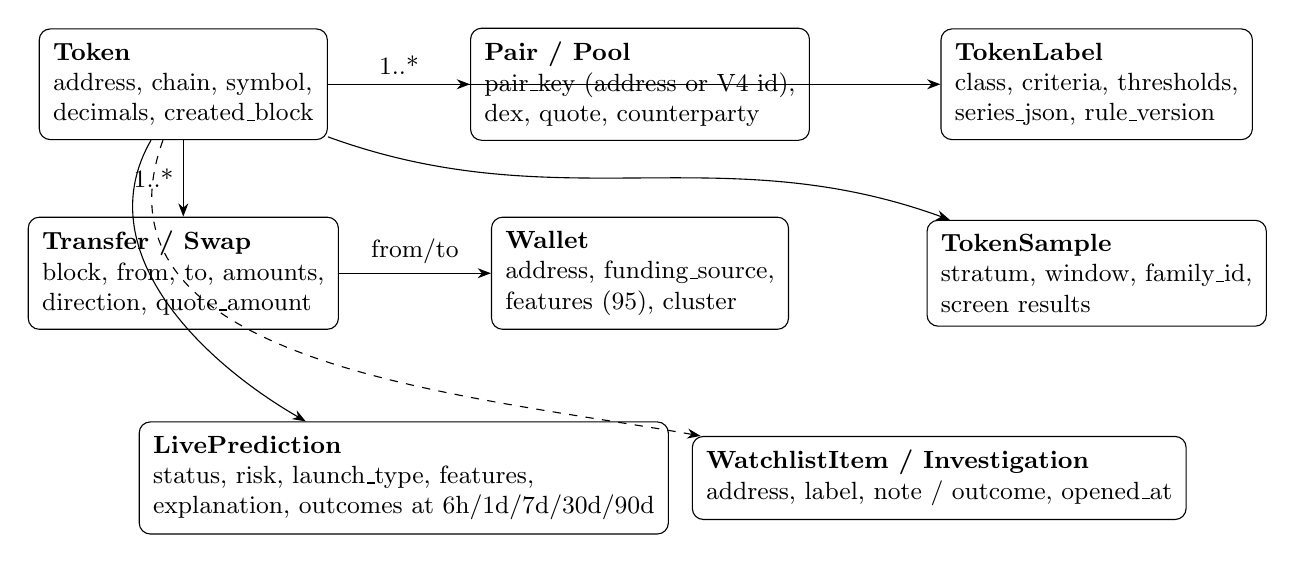
\begin{tikzpicture}[font=\small, ent/.style={draw, rounded corners, align=left, inner sep=5pt}, >={Stealth}]
  \node[ent] (token) at (0,0) {\textbf{Token}\\address, chain, symbol,\\decimals, created\_block};
  \node[ent] (pair) at (5.8,0) {\textbf{Pair / Pool}\\pair\_key (address or V4 id),\\dex, quote, counterparty};
  \node[ent] (transfer) at (0,-2.4) {\textbf{Transfer / Swap}\\block, from, to, amounts,\\direction, quote\_amount};
  \node[ent] (wallet) at (5.8,-2.4) {\textbf{Wallet}\\address, funding\_source,\\features (95), cluster};
  \node[ent] (label) at (11.6,0) {\textbf{TokenLabel}\\class, criteria, thresholds,\\series\_json, rule\_version};
  \node[ent] (sample) at (11.6,-2.4) {\textbf{TokenSample}\\stratum, window, family\_id,\\screen results};
  \node[ent] (pred) at (2.8,-5) {\textbf{LivePrediction}\\status, risk, launch\_type, features,\\explanation, outcomes at 6h/1d/7d/30d/90d};
  \node[ent] (prod) at (9.6,-5) {\textbf{WatchlistItem / Investigation}\\address, label, note / outcome, opened\_at};
  \draw[->] (token) -- node[above]{1..*} (pair);
  \draw[->] (token) -- node[left]{1..*} (transfer);
  \draw[->] (transfer) -- node[above]{from/to} (wallet);
  \draw[->] (token) -- (label);
  \draw[->] (token) to[out=-20,in=160] (sample);
  \draw[->] (token) to[out=-120,in=150] (pred);
  \draw[->, dashed] (token) to[out=-110,in=170] (prod);
\end{tikzpicture}\end{adjustbox}
\caption{Domain model. A token has pools, transfers and swaps; wallets are the transfer endpoints; a label and a sample row describe how the token entered the dataset and what happened to it; a live prediction is written once per launch the feed judged.}
\end{figure}

\section{Data Design}
The store has sixteen tables under Alembic migrations (ten revisions). The ingestion tables (\code{token}, \code{pair}, \code{pair_snapshot}, \code{transfer}, \code{swap}, \code{wallet}, \code{ingest_run}, \code{budget_ledger}, \code{backfill_checkpoint}) use unconstrained \code{NUMERIC} for amounts and prices because real Base data overflowed a fixed precision on the day it was written and a dust price rounded to zero without complaint. \code{token_label} stores its observations (\code{series_json}) so every verdict can be re-derived offline; \code{rule_version} is part of its key so a changed threshold writes a new generation. \code{token_sample} carries the stratum every headline number depends on. \code{live_prediction} is append-only by construction (\code{ON CONFLICT DO NOTHING}) and holds the features and the explanation beside the prediction. \code{watchlist_item} and \code{investigation} are the product's state. Every write is an upsert on a natural key, batched at 5,000 rows, and reports inserts and updates separately so a re-run can be proved to write zero new rows.

\section{Process / Behavior Design}
\begin{figure}[H]
\centering
\begin{adjustbox}{max width=\textwidth}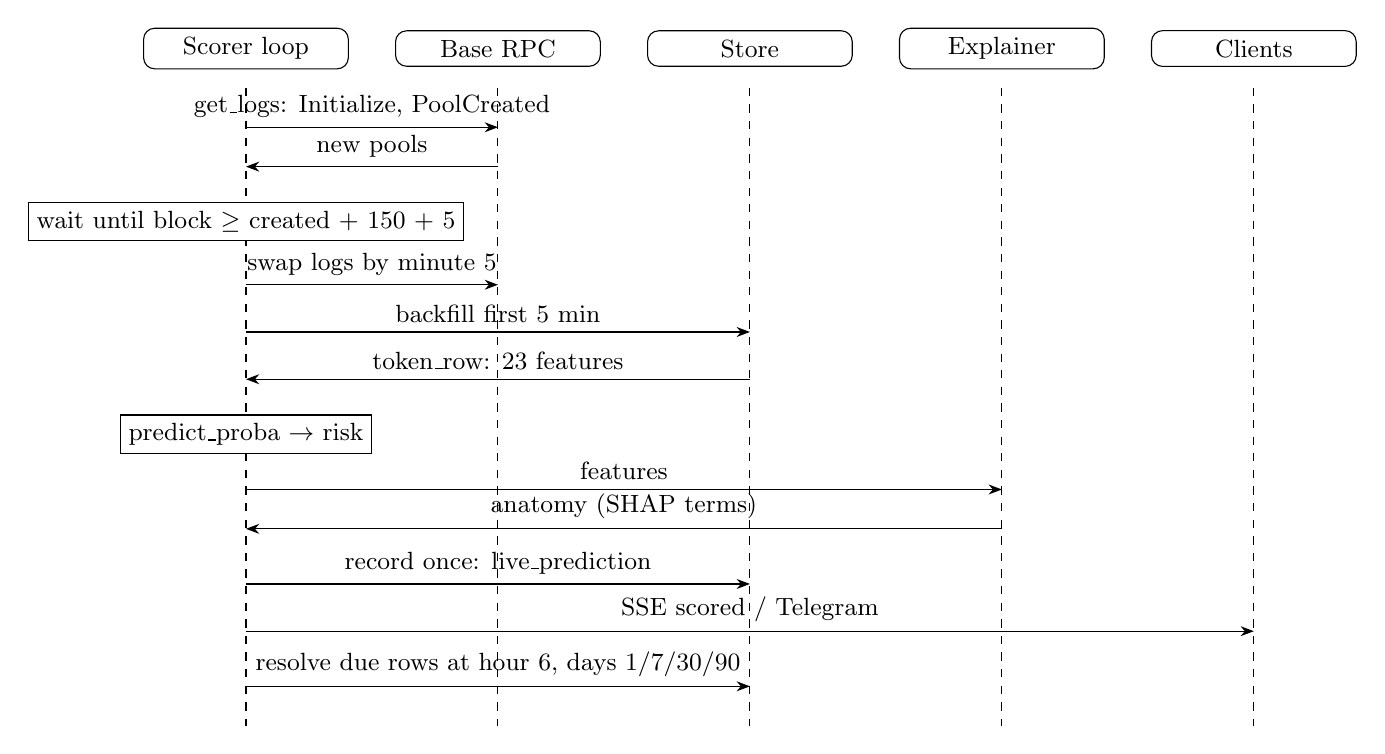
\begin{tikzpicture}[font=\small, >={Stealth}, every node/.style={align=center}]
  \foreach \x/\n in {0/Scorer loop, 3.2/Base RPC, 6.4/Store, 9.6/Explainer, 12.8/Clients}
    { \node[draw, rounded corners, minimum width=2.6cm] (h\n) at (\x,0) {\n}; \draw[dashed] (\x,-0.5) -- (\x,-8.6); }
  \draw[->] (0,-1) -- node[above]{get\_logs: Initialize, PoolCreated} (3.2,-1);
  \draw[->] (3.2,-1.5) -- node[above]{new pools} (0,-1.5);
  \node[draw, fill=white, inner sep=3pt] at (0,-2.2) {wait until block $\geq$ created + 150 + 5};
  \draw[->] (0,-3) -- node[above]{swap logs by minute 5} (3.2,-3);
  \draw[->] (0,-3.6) -- node[above]{backfill first 5 min} (6.4,-3.6);
  \draw[->] (6.4,-4.2) -- node[above]{token\_row: 23 features} (0,-4.2);
  \node[draw, fill=white, inner sep=3pt] at (0,-4.9) {predict\_proba $\to$ risk};
  \draw[->] (0,-5.6) -- node[above]{features} (9.6,-5.6);
  \draw[->] (9.6,-6.1) -- node[above]{anatomy (SHAP terms)} (0,-6.1);
  \draw[->] (0,-6.8) -- node[above]{record once: live\_prediction} (6.4,-6.8);
  \draw[->] (0,-7.4) -- node[above]{SSE scored / Telegram} (12.8,-7.4);
  \draw[->] (0,-8.1) -- node[above]{resolve due rows at hour 6, days 1/7/30/90} (6.4,-8.1);
\end{tikzpicture}\end{adjustbox}
\caption{Sequence of one scorer tick (every 60 s).}
\end{figure}

\begin{figure}[H]
\centering
\begin{adjustbox}{max width=\textwidth}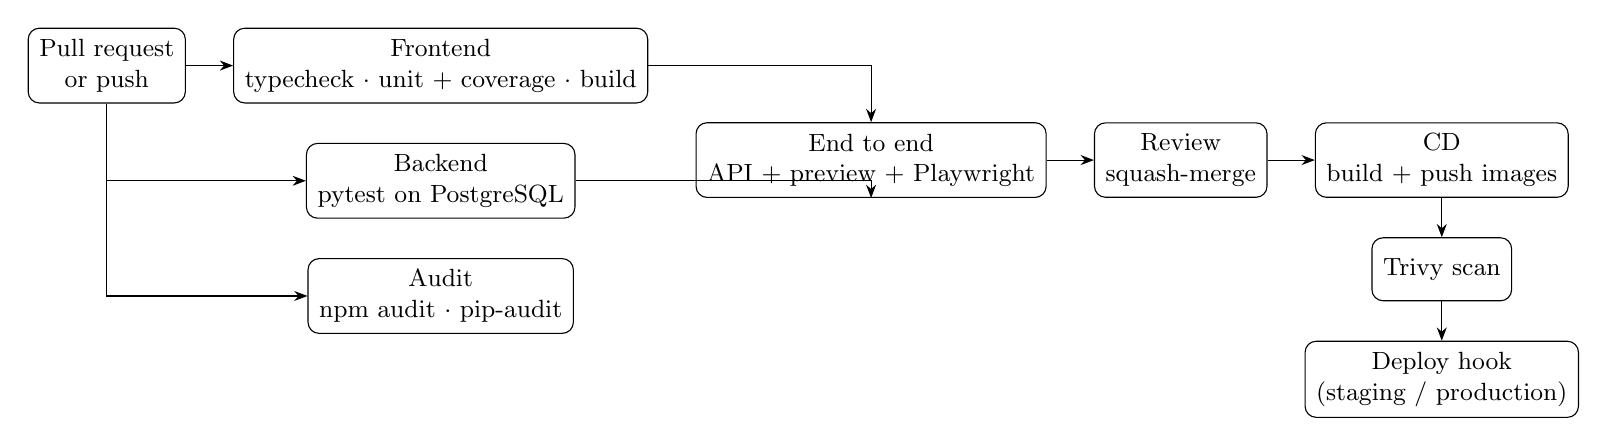
\begin{tikzpicture}[font=\small, >={Stealth}, stage/.style={draw, rounded corners, align=center, minimum height=0.8cm, inner sep=4pt}, node distance=0.5cm and 0.6cm]
  \node[stage] (pr) {Pull request\\or push};
  \node[stage, right=of pr] (fe) {Frontend\\typecheck $\cdot$ unit + coverage $\cdot$ build};
  \node[stage, below=of fe] (be) {Backend\\pytest on PostgreSQL};
  \node[stage, below=of be] (au) {Audit\\npm audit $\cdot$ pip-audit};
  \node[stage, right=of fe, yshift=-1.2cm] (e2e) {End to end\\API + preview + Playwright};
  \node[stage, right=of e2e] (merge) {Review\\squash-merge};
  \node[stage, right=of merge] (img) {CD\\build + push images};
  \node[stage, below=of img] (scan) {Trivy scan};
  \node[stage, below=of scan] (dep) {Deploy hook\\(staging / production)};
  \draw[->] (pr) -- (fe); \draw[->] (pr) |- (be); \draw[->] (pr) |- (au);
  \draw[->] (fe) -| (e2e); \draw[->] (be) -| (e2e);
  \draw[->] (e2e) -- (merge); \draw[->] (merge) -- (img); \draw[->] (img) -- (scan); \draw[->] (scan) -- (dep);
\end{tikzpicture}\end{adjustbox}
\caption{The delivery pipeline.}
\end{figure}

\chapter{Iteration 1: Design and Implementation}
\label{ch:iter1}

\section{Iteration Objectives}
Prove that a free, keyless data path can discover, store and label Base launches; find whether anything observable at launch predicts the outcome; put whatever survives validation into a live service; and build the interface the proposal showed. Iteration 2 (Chapter~\ref{ch:test} onwards) then proved the signal forward and built the product around it.

\section{Selected Use Cases / Features}
UC1 (watch launches), UC3 (investigate), UC7 (forward record, groundwork), UC9 (trending), and the research pipeline behind FR-1 and FR-2.

\section{Design}
The backend is a set of phases that each read the store and write back through one gate (Figure~\ref{fig:arch}). The phases are separable: ingestion can run without labels, labels without models, and the live scorer uses the same feature code as training (\code{token_features.token_row}) so a live score is computed the way the validated one was. The front end is data-separated: no component invents a value; it renders records from \code{src/data/} or from the API.

\section{Implementation}
\textbf{Phase 1} (11 October) built the package, config, schema and ingestion; the acceptance run backfilled 159 complete 24-hour windows (64,354 transfers, 15,628 swaps, 12,158 wallets) at a measured 44 calls per window and cost nothing. \textbf{Phase 2} (13 October) defined the labels and swept every threshold. \textbf{Phase 3} built the wallet graph (14,528 funding edges, 111,705 co-purchase edges, 134 provable clusters) and validated co-movement lift (4.66, $p = 1.3\times10^{-5}$). \textbf{Phase 4} trained a first model and \textbf{Phase 5 Part A} (18 October) audited it and withdrew it. \textbf{Phase 5 Parts B--D} redesigned the sample (1,066 alive tokens, 841 families, 297,000 keyless calls) and retrained; \textbf{Phase 6} split FAILED and found the buyer-loss target; \textbf{Phase 7} (19 October) shipped the API and the live feed.

\section{Completed Features / Module}
\begin{itemize}
  \item Chain-event discovery and resumable windowed backfill, with budgets and a lookahead-proof write gate.
  \item Outcome labels with stored observations and an offline sensitivity sweep.
  \item A properly sampled dataset with operator families and a data card.
  \item Two validated signals and a shipped artefact with its validation record.
  \item A live scorer and FastAPI service; the Fresh Launches page; the live Trending page; the token page.
\end{itemize}

\section{Technical Implementation Details}
\begin{table}[H]
\centering\small
\begin{tabular}{p{0.34\textwidth}p{0.57\textwidth}}
\toprule
File & What it holds\\
\midrule
\code{blocklens/config.py} & every tunable from the environment: sources, caps, budgets, alert settings\\
\code{blocklens/store/write.py} & the write gate: \code{LookaheadError}, batched upserts, coalescing of nullable columns, product-state writers\\
\code{blocklens/ingest/chain.py} & \code{discover_pools}, \code{backfill_token}: V4 \code{Initialize} and V3 \code{PoolCreated}, 1,000-block windows, V4 swaps by topic filter\\
\code{blocklens/label/rules.py} & named criteria and thresholds; \code{LIQUIDITY_DROP_FRACTION = 0.90}, 90-day window\\
\code{blocklens/label/sample.py} & \code{balanceOf} and \code{extsload} at historical blocks; the V4 token-side method\\
\code{blocklens/sampling/design.py} & windows, strata, families, \code{CUTOFF_BLOCKS = 150} (five minutes)\\
\code{blocklens/model/token_features.py} & the 23 features of \code{t5-2026-10}\\
\code{blocklens/live/scorer.py} & the loop: discover, screen, backfill, score, explain, alert, record, resolve, prune\\
\code{blocklens/live/explain.py} & tree SHAP decomposition, labels, display units\\
\code{blocklens/live/resolver.py} & append-only record, outcomes, scoreboard, paper agent, trade book\\
\code{blocklens/api/app.py} & fourteen endpoints, a session dependency, the SSE generator\\
\code{src/lib/live/*.ts} & typed readers for the API and the public sources; pure arithmetic for the paper book and health\\
\code{src/routes/Launches.tsx} & the feed, push, toasts, notifications, the why-drawer\\
\bottomrule
\end{tabular}
\caption{Key implementation files.}
\end{table}

\section{Algorithms and Technical Decisions}
\begin{description}
  \item[The label.] RUG if the token-side reserve fell by $\geq 90\%$ between consecutive samples within 90 days; FAILED if the price collapsed or trading stopped without a reserve collapse; SURVIVED if it still holds $\geq 25\%$ of peak liquidity and traded on $\geq 8$ of the last 30 days; UNCLEAR below 80\% usable samples; NEVER\_LAUNCHED if it never traded or the pool is degenerate. Each criterion is a named boolean and the verdict one expression, so the sweep can move any threshold.
  \item[Case-control sampling.] A nine-point coarse reserve read (18 calls) selects cases (91\% turn out RUG); a 20\% Bernoulli draw of the rest gives controls; the random cohort, outcome-blind, is the only set at true prevalence and the only evaluation set.
  \item[The model.] \code{HistGradientBoostingClassifier} (depth 3, 300 iterations, learning rate 0.05, L2 = 1.0), Platt-scaled, trained on 593 labelled non-RUG tokens alive at minute 5; a logistic regression is reported beside it. Splits are grouped by family; every confidence interval resamples families.
  \item[Explanations.] Path-dependent TreeSHAP~\cite{lundberg2020} on the shipped ensemble gives one log-odds term per feature; the terms plus the base value equal the model's logit, which a test asserts.
  \item[Budgets.] A token bucket per source (DexScreener 60/min, RPC 4/s, burst 4), a per-run call ceiling, and a persisted monthly ledger.
  \item[Communities.] Louvain with a fixed seed, after greedy modularity failed to finish on 15,000 nodes.
\end{description}

\section{Tools, Frameworks and Technologies}
Python 3.12, FastAPI, uvicorn, SQLAlchemy 2, Alembic, PostgreSQL 16 with TimescaleDB, httpx, scikit-learn, numpy, scipy, networkx, shap, joblib, pytest, pytest-cov; TypeScript 5, React 18, React Router 6, Vite 5, vitest, Playwright; Docker, nginx, GitHub Actions, GHCR, Trivy, Dependabot; TinyTeX for this report.

\section{Demonstration Evidence}
\textbf{The product is deployed and open to anyone:} \url{https://flying-boron-kxx29gy.tmp.now}.
The repository, which always carries the current address, is \url{https://github.com/AbdullahBinNasir16/BlockLens}.

The landing page, the three case studies, Trending Tokens and the wallet screener run entirely in the browser. Fresh Launches, the token page's signals, Paper Agent and Model Health read the BlockLens API, so they report the API as unreachable unless the API is running: during the demonstration it is started with \code{uvicorn blocklens.api.app:app --port 8000}, and the figures below were captured against it. Hosting the API itself is module M11 (Section~\ref{sec:roadmap}).

\begin{figure}[H]\centering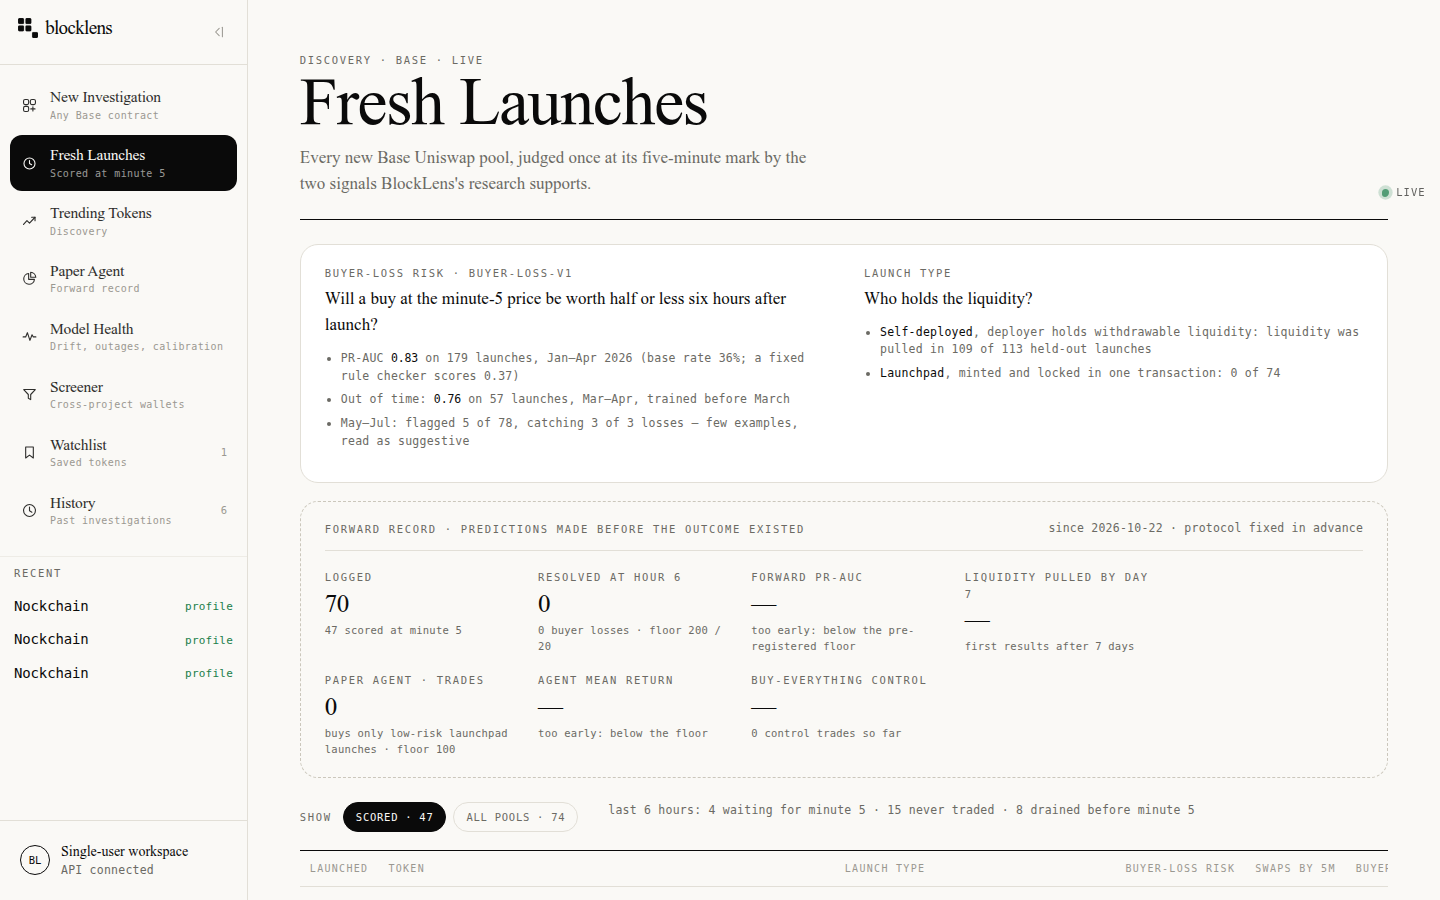
\includegraphics[width=\textwidth]{figures/launches.png}\caption{Fresh Launches: every new Base pool scored at minute 5, with the validation record, the forward record, push status and the why-button.}\end{figure}
\begin{figure}[H]\centering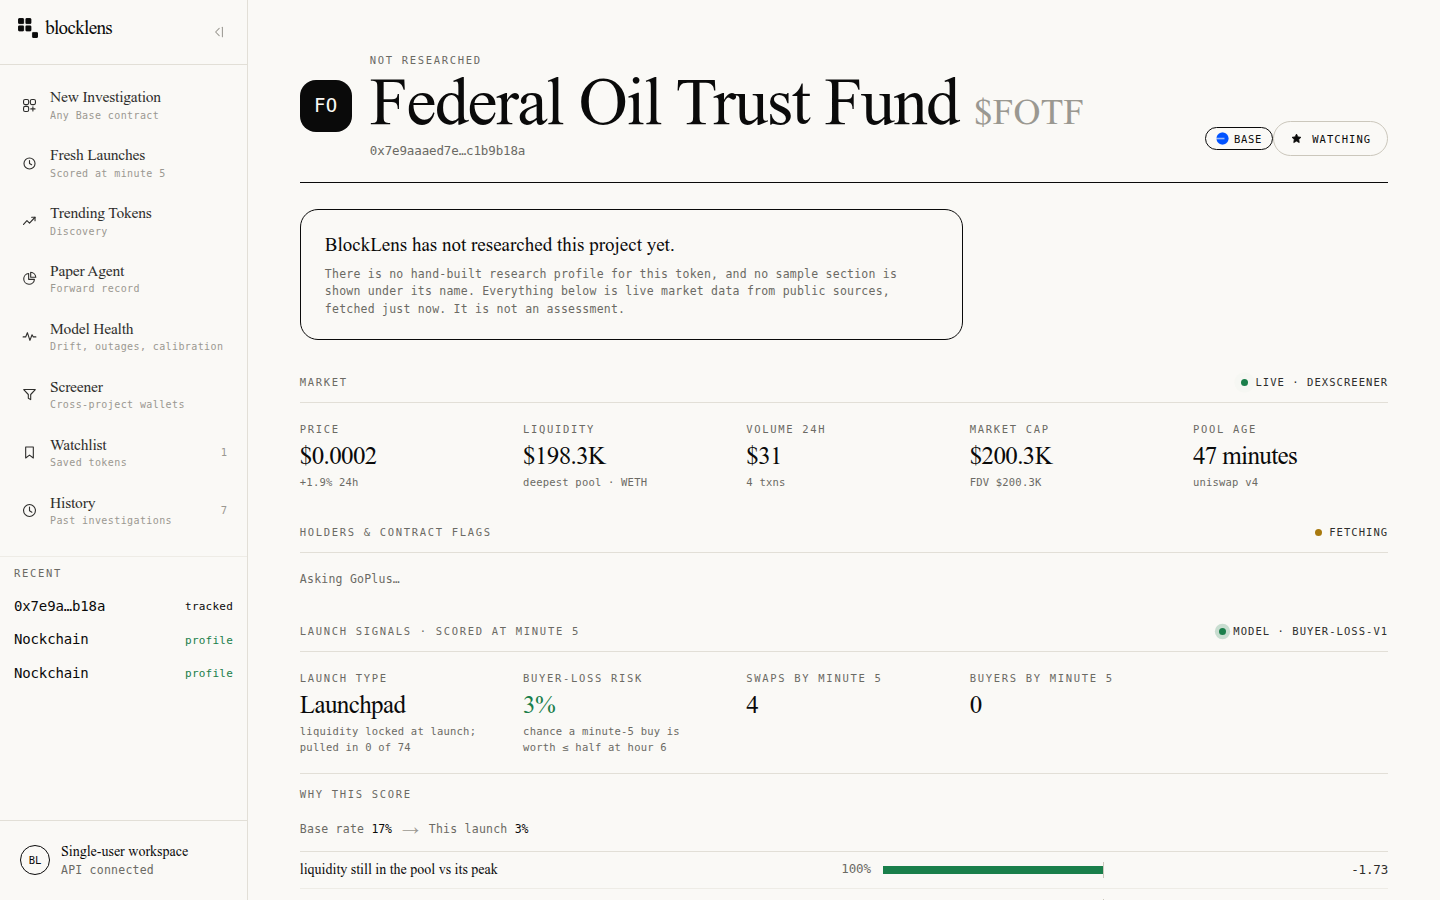
\includegraphics[width=\textwidth]{figures/token.png}\caption{The token page for a tracked launch: live market data, GoPlus flags, the two signals and the score's anatomy.}\end{figure}
\begin{figure}[H]\centering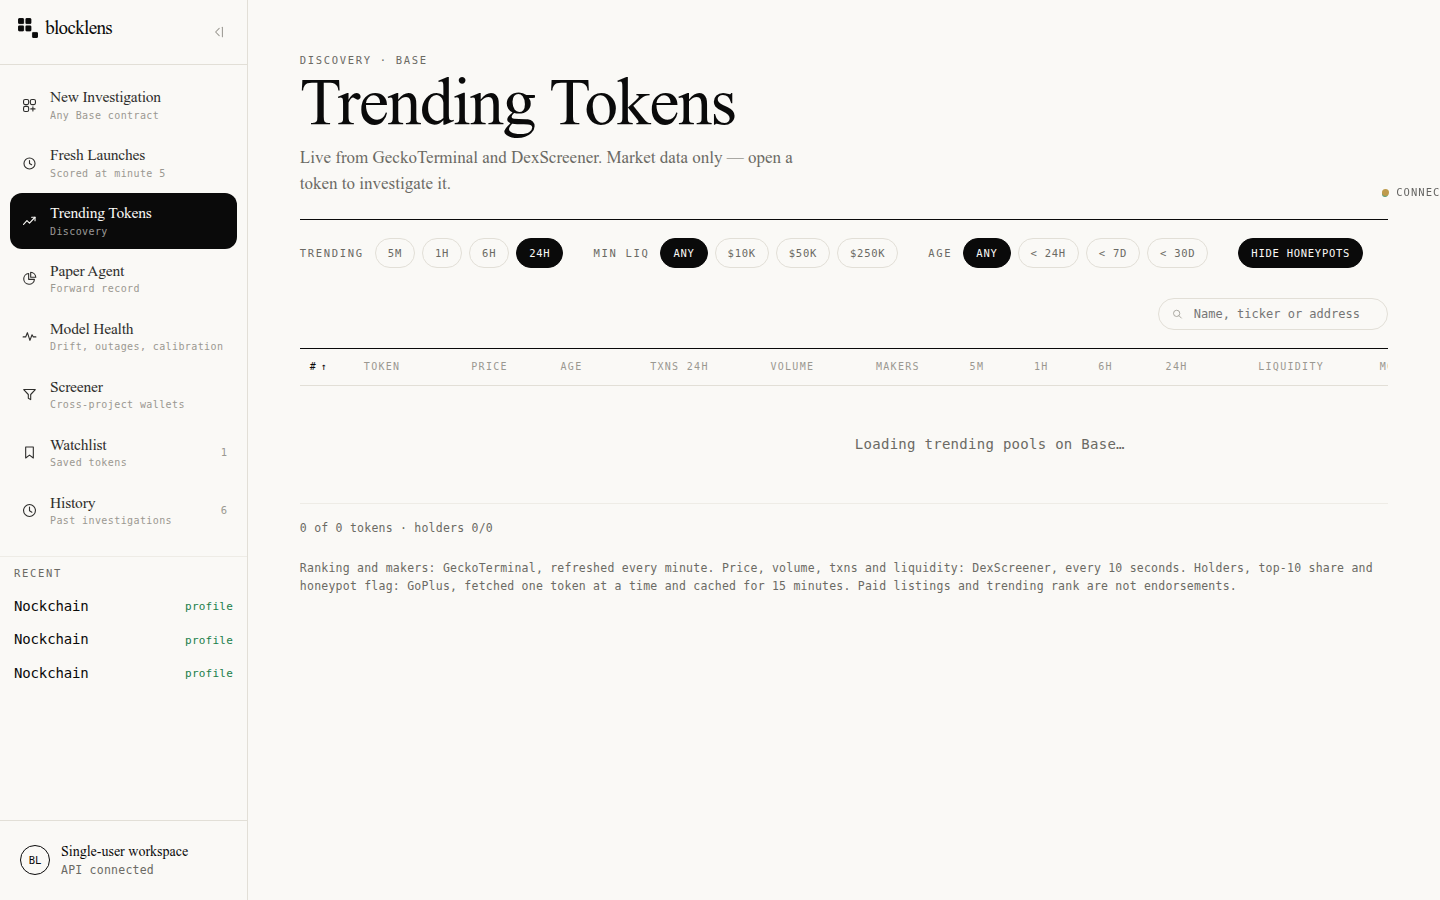
\includegraphics[width=\textwidth]{figures/trending.png}\caption{Trending Tokens over live Base pools.}\end{figure}

\section{Iteration Outcome}
The data path works and costs nothing; the labels are defensible; the first model's result was wrong and was replaced by two signals that hold up out of time; the live feed judges launches within a minute of their five-minute mark. The iteration also produced the project's most important negative result: the wallet graph, which the proposal built on, adds nothing measurable on this population.

\chapter{Testing and Early Validation}
\label{ch:test}

\section{Testing Strategy}
Three layers, each with a rule that makes a passing test mean something. \textbf{Unit and API tests} run with the network transport blocked for the whole backend suite, so a test that leaks a real call fails instead of passing against a live API; store tests run on a real PostgreSQL because the idempotency proof depends on PostgreSQL-specific SQL. \textbf{End-to-end tests} drive the built bundle in a real browser against the real API on a PostgreSQL service. \textbf{Validation} of the model is pre-registered: baselines, metrics, floors and success criteria are written before the data is seen, and the forward test logs every prediction before its outcome exists.

\section{Test Levels and Techniques}
\begin{table}[H]
\centering\small
\begin{tabular}{p{0.14\textwidth}p{0.36\textwidth}p{0.34\textwidth}}
\toprule
Level & Technique & Where\\
\midrule
Unit (backend) & recorded fixtures via \code{httpx.MockTransport}; property-style checks (additivity, idempotency, determinism) & \code{backend/tests/}, 158 functions\\
Unit (frontend) & pure functions with fixed inputs; the README's acceptance query as a test & \code{src/**/*.test.ts}, 33 cases\\
API & FastAPI \code{TestClient} with a rolled-back session injected by dependency override & \code{test_api.py}, \code{test_product_api.py}\\
End to end & Playwright, Chromium, real API & \code{e2e/smoke.spec.ts}, 7 cases\\
Static & TypeScript strict mode, \code{noUnusedLocals}; \code{DeprecationWarning} as error in pytest & CI\\
Security & \code{npm audit}, \code{pip-audit}, Trivy on images & CI, CD\\
Data integrity & SQL checks on the stored rows: 0 transfers after \code{as_of_ts}, 0 before creation, byte-identical re-ingest & Phase 1 acceptance\\
Validation & held-out random cohort, out-of-time split, permutation nulls, family bootstrap, pre-registered checkers, forward record & \code{backend/reports/}\\
\bottomrule
\end{tabular}
\caption{Test levels and techniques.}
\end{table}

\section{Test Cases}
Selected cases; the full list is in Appendix~\ref{app:tests}.
\begin{table}[H]
\centering\small
\begin{tabular}{p{0.08\textwidth}p{0.46\textwidth}p{0.3\textwidth}p{0.08\textwidth}}
\toprule
ID & Case & Expected & Result\\
\midrule
T-01 & Write a batch with one row later than \code{as_of_ts} & \code{LookaheadError}, nothing written & pass\\
T-02 & Re-ingest a complete token with checkpoints deleted & zero inserts, same MD5 over rows & pass\\
T-03 & Enrichment runs after chain ingest & \code{decimals} kept (coalesce), name filled & pass\\
T-04 & Louvain three times on the same graph & identical assignments & pass\\
T-05 & Explain three feature rows & terms + base = model logit within 1e-3; rest = 0 & pass\\
T-06 & Notifier with no configuration & \code{send} returns False, no network & pass\\
T-07 & Notifier with a mock transport & POST to \code{api.telegram.org} with chat id and risk & pass\\
T-08 & \code{POST /api/watchlist} twice, then \code{DELETE} & created then updated; label coalesced; 404 on second delete & pass\\
T-09 & \code{GET /api/stream?ticks=1} & \code{event: hello} then \code{: ping} & pass\\
T-10 & \code{GET /api/token/not-an-address} & 400 & pass\\
T-11 & Acceptance screener query over the seeded corpus & exactly 8 wallets, each with $\geq 2$ matched projects & pass\\
T-12 & Unknown check id in a screener query & zero matches (fails closed) & pass\\
T-13 & Paper book stats on a four-trade fixture & mean, median, hit rate, pulled count as computed by hand & pass\\
T-14 & Browser: paste an unknown address & lands on the live token page, not a profile & pass\\
T-15 & Browser: watchlist round trip through the API & row visible, then removed & pass\\
\bottomrule
\end{tabular}
\caption{Selected test cases.}
\end{table}

\section{Test Results}
\begin{table}[H]
\centering\small
\begin{tabular}{lrrl}
\toprule
Suite & Cases & Result & Where\\
\midrule
Backend pytest (PostgreSQL service) & 161 & 161 passed & CI, PR \#2 and later\\
Frontend vitest & 33 & 33 passed, coverage floor met & CI\\
Playwright end to end & 7 & 7 passed & local and CI (PR \#4)\\
TypeScript strict typecheck & -- & 0 errors & CI\\
\bottomrule
\end{tabular}
\caption{Test results at the time of writing (22 October 2026).}
\end{table}

\section{Acceptance Testing / Validation}
\begin{table}[H]
\centering\small
\begin{tabular}{p{0.3\textwidth}p{0.2\textwidth}p{0.2\textwidth}p{0.22\textwidth}}
\toprule
Measurement & BlockLens & Baseline & Set\\
\midrule
Liquidity-pull: self-deployed pulled & 109 of 113 & -- & EVAL random cohort\\
Liquidity-pull: launchpad pulled & 0 of 74 & -- & EVAL random cohort\\
Buyer-loss PR-AUC, in period & 0.833 & 0.370 (checker) & CAL, 179 tokens, base rate 0.36\\
Buyer-loss PR-AUC, out of time & 0.758 & 0.331 & Mar--Apr, trained before Mar\\
Regime check May--Jul & 5 flagged of 78, all 3 losses caught & -- & few examples\\
Forward resolved predictions & 850 & floor 200 / 20 losses (14 so far) & since 19 Oct\\
Paper agent mean return & $+49.3\%$ (315 trades) & $-33.4\%$ control (832) & CI $+55\%$ to $+110\%$\\
Self-deployed pulled within a day (forward) & 86\% & 0.4\% launchpad & forward\\
\bottomrule
\end{tabular}
\caption{Validation results. Sources: \codex{model\_card\_v2.md}, \codex{model\_card\_phase6.md}, \codex{paper\_agent.md}.}
\end{table}
The paper agent's pre-registered success criterion is met. The buyer-loss forward record is below its floor for losses and no forward accuracy claim is made; the page shows the counts and says ``too early''.

\section{Edge and Failure Cases}
\begin{itemize}
  \item A token minting $10^{30}$ units overflowed \code{NUMERIC(38,18)} and a dust price rounded to zero in \code{NUMERIC(38,12)}: both columns are now unconstrained.
  \item The first failed run left no record because the bookkeeping wrote to an aborted session; the runner now rolls back before recording a failure.
  \item A stopped database made the suite hang rather than skip; the engine fixture now has a 3-second connect timeout.
  \item A V4 pool keyed by id never matched a transfer counterparty, silently emptying a join and nearly producing a false ``no co-movement'' finding.
  \item A 107,000-row upsert did not finish; writes are batched at 5,000.
  \item RPC 403/429: PublicNode rate-banned a probe after four minutes; the budget module keeps the project under measured limits.
  \item Outage: late-due launches are logged as missed; a catch-up backlog was found to delay live launches and was removed.
\end{itemize}

\section{Defects and Corrective Actions}
\begin{table}[H]
\centering\small
\begin{tabular}{p{0.4\textwidth}p{0.51\textwidth}}
\toprule
Defect & Correction\\
\midrule
Phase 4 model learned the label (64/85 leaking features; total censoring) & model withdrawn; 5-minute window; redesigned sampling; family splits\\
\code{SET col = excluded.col} erased correct decimals on enrichment & nullable columns coalesce; caught by a test\\
Age decided by DexScreener timestamp let a 369-day-old token through & age by block number\\
Failed \code{balanceOf} swallowed, giving a confident verdict on 12/112 samples & failures recorded; $<80\%$ usable $\to$ UNCLEAR\\
Prior-shift correction made the logistic model worse on EVAL & reported, not dropped; boosting with Platt scaling shipped\\
Scoring a 38-hour backlog delayed live launches & launches past their 6-hour mark are logged as missed, never scored\\
Stacked pull requests ran no CI (trigger limited to \code{main}/\code{develop}) & CI runs on every pull request and on feature branches\\
Playwright strict-mode locator collisions (two ``Open Workspace'' links; name in table and sidebar) & locators scoped to the navigation and the table\\
\code{pip-audit} in CI flagged twelve known vulnerabilities in Starlette 0.48, pinned by FastAPI 0.118 & FastAPI upgraded to 0.159 (Starlette 1.9); suite unchanged; re-audit clean. The gate found a real issue on its first run\\
\bottomrule
\end{tabular}
\caption{Defects found and corrected.}
\end{table}

\section{Current Validation Status}
All automated suites pass in CI. The model's held-out and out-of-time validation is complete and shipped with every score. The forward test is running; its liquidity-pull half is already decisive forward (86\% vs 0.4\% within a day), its buyer-loss half awaits its floor, and the paper agent has passed its floor with a positive, robust margin whose source the product names honestly.

\chapter{Project Management and Development Evidence}
\label{ch:pm}

\section{Work Completed}
Modules M1 to M6 (Section~\ref{sec:scope}) are implemented, tested and running; the forward test and paper agent have produced their first reportable result; the CI/CD pipeline runs on every pull request and publishes images; the product has been narrowed to what the research defends; this report exists under version control and is compiled by the pipeline.

\section{Work Remaining}
Branch protection to be switched on by the repository owner; the first 7-day liquidity results of the forward test (due 26 October 2026); hosting of the compose stack on a server; the FYP-2 modules M7--M11 (Chapter~\ref{ch:plan}); the proposal action register and meeting records to be completed from the team's own forms.

\section{Individual Responsibilities}
\begin{itemize}
  \item \textbf{Abdullah Bin Nasir:} data research (feasibility spikes, ingestion, labels, graph, sampling, models), the live scorer, forward validation and paper agent protocols, the decision log, the front-end prototype and design system.
  \item \textbf{Shahmir Khan Lughmani:} delivery engineering (CI/CD, containers, test strategy and the unit, API and end-to-end suites), the Phase 10 API features (explanations, alerts, health, product state), the product rework and scope document, this report.
  \item \todo{Third member's responsibilities, if any.}
\end{itemize}

\section{Contribution of Each Team Member}
\begin{table}[H]
\centering\small
\begin{tabular}{p{0.3\textwidth}rp{0.47\textwidth}}
\toprule
Member & Commits & Principal artefacts\\
\midrule
Abdullah Bin Nasir & 24 & \code{backend/blocklens/{ingest,label,graph,sampling,model,live}}, \code{scripts/}, \code{reports/}, \code{DECISIONS.md} Phases 1--9, \code{src/} prototype\\
Shahmir Khan Lughmani & 12+ & \code{.github/}, \code{Dockerfile}s, \code{docker-compose.prod.yml}, \code{e2e/}, \code{src/**/*.test.ts}, \code{live/explain.py}, \code{alerts.py}, \code{health.py}, Phase 10 API and migration, \code{src/routes/{Portfolio,ModelHealth,Watchlist,History}}, \code{docs/FYP1_SCOPE.md}, \code{CONTRIBUTING.md}, \code{report/}\\
\todo{Third member} & & \\
\bottomrule
\end{tabular}
\caption{Contributions by member, from \codex{git shortlog} on 22 October 2026. \todo{Update the counts at submission.}}
\end{table}

\section{Repository and Version Control Evidence}
Repository: \code{github.com/AbdullahBinNasir16/BlockLens} (private; the panel has access). Branches: \code{main} (release), \code{develop} (integration), \code{feature/ci-cd-pipeline}, \code{feature/phase10-backend}, \code{feature/product-rework}, \code{feature/ci-hardening}, each with a pull request that CI checks. Commit messages follow conventional prefixes with a body that says why. Pull requests use the template in \code{.github/pull_request_template.md}. Appendix~\ref{app:repo} lists the pull requests and CI runs.

\section{Milestones and Commit Evidence}
\begin{table}[H]
\centering\small
\begin{tabular}{llp{0.53\textwidth}}
\toprule
Date & Commits & Milestone\\
\midrule
09--10 Sep 2026 & 9 & front-end prototype: design system, landing, shell, profiles, screener, directory, portfolio\\
11 Oct & 3 & feasibility spikes; Phase 1 package, schema, ingestion\\
13 Oct & 3 & labels; Phase 3 graph; Phase 4 model\\
18 Oct & 5 & leakage audit; sampling design; Phase 5 retrain; buyer-loss model\\
19 Oct & 2 & live scorer, resolver, FastAPI; Fresh Launches\\
21 Oct & 2 & paper agent passes its floor; README, backend guide, decision log\\
22 Oct & 12 & CI/CD, tests, containers, scope; Phase 10 backend; product rework; CI hardening; report\\
\bottomrule
\end{tabular}
\caption{Milestones and commit counts from the git history.}
\end{table}

\section{Tools and Tool-Assisted Development}
\label{sec:tools}
Development tools: VS Code, git and the GitHub CLI, uv and pip, npm, Docker (in CI), PostgreSQL 16, TinyTeX. Process tools: GitHub pull requests, Actions, Dependabot, GHCR, Trivy.

\textbf{AI assistance, disclosed.} An AI coding assistant (Claude Code, Anthropic) was used during development as a pair-programming and drafting tool, under the team's direction: to draft code and tests that the team then ran, reviewed and committed; to draft documentation from the repository's own records; and to draft this report from \code{DECISIONS.md}, the model cards and the code. Every measurement in the report was produced by the project's own scripts; every design decision was taken by the team and is recorded with its evidence. Commits made with the assistant carry a co-author trailer so the history is honest about it. The team considers this the same category of tool as a compiler or a linter: it speeds the work and does not stand in for understanding it, which the viva will test.

\section{External Components and Dependencies}
Keyless public endpoints (Tenderly gateway, DexScreener, GeckoTerminal, GoPlus, optionally Telegram) and the open-source libraries listed in Chapter~\ref{ch:design}, pinned in \code{backend/pyproject.toml} and \code{package-lock.json} and audited on every pull request. The project's own model artefact (\code{buyer_loss_v1.joblib}) is versioned in the repository with its metadata. Third-party marks (token and chain logos, X profile pictures) are used only to identify the projects they belong to.

\section{Risks and Mitigation}
\begin{table}[H]
\centering\small
\begin{tabular}{p{0.34\textwidth}p{0.1\textwidth}p{0.40\textwidth}}
\toprule
Risk & Likelihood & Mitigation\\
\midrule
A free endpoint changes its limits or goes keyed & high (two already did) & measured fallbacks (\code{rpc_fallback_url}); GoPlus replaced Blockscout; budgets keep usage polite\\
Forward test interrupted (one machine) & high & auto-start task; late launches logged as missed, never scored; hosting in FYP-2\\
Regime shift degrades calibration & medium & Model Health tracks the self-deployed share; retrain on the forward record (M10)\\
Buyer-loss forward floor not reached before evaluation & medium & the page reports counts and says ``too early''; the launch-type half is already decisive\\
Scope creep back toward unmeasurable features & medium & \code{docs/FYP1_SCOPE.md}; every number labelled Sourced / Sample\\
Dependency vulnerability & medium & audits on PRs, Trivy on images, Dependabot weekly\\
Key person risk (research in one member's head) & medium & the decision log and model cards; this report; shared ownership of the live code through PRs\\
\bottomrule
\end{tabular}
\caption{Risks and mitigations.}
\end{table}

\section{Security and Privacy Considerations}
No secrets in the repository; the only credential the system can hold (a Telegram bot token) is read from the environment and never logged. All inbound addresses are validated server-side. The write gate and append-only prediction log make tampering with the forward record a visible change in git and in the database. The system stores only public chain data and groups pseudonymous addresses; it holds no personal data, and the product's own state (watchlist, history) is local to one deployment.

\section{Current Limitations}
\begin{itemize}
  \item One chain, one DEX family (Uniswap V3/V4).
  \item The forward test depends on a single machine until hosted.
  \item The wallet screener still runs over a generated corpus, labelled as such, until M9.
  \item No accounts: one watchlist per deployment.
  \item The buyer-loss model should not be used on launchpad tokens as a rug predictor (its answer there is always ``not pulled'', which is true and useless); the page reads liquidity-pull risk from launch type.
  \item Prices in the store are ratios against each token's quote asset; dollar PnL needs an ETH/USD series (M9).
\end{itemize}

\chapter{Remaining FYP Plan}
\label{ch:plan}

\section{Remaining Scope}
The FYP-2 scope is the set M7--M11 of \code{docs/FYP1_SCOPE.md}: one investigation flow, richer persistence, an early-buyer screener over stored transfers, a model retrained on the forward record, and hosting. Nothing cut in FYP-1 returns unless a free, measured source for it appears.

\section{Remaining Modules and Features}
\begin{table}[H]
\centering\small
\begin{tabular}{p{0.06\textwidth}p{0.3\textwidth}p{0.52\textwidth}}
\toprule
\# & Module & Definition of done\\
\midrule
M7 & One investigation flow & \code{/app/new} resolves any Base address to the token page; the case studies are reached from a ``Case studies'' link; the research animation is retired\\
M8 & Persistence & notes on watchlist items; alert preferences; history filters; export of the forward record as CSV\\
M9 & Early-buyer screener & ``which wallets bought tracked launches in their first six hours and what did they realise'' over the backend's transfers and swaps; \code{evaluateQuery} becomes a POST; an ETH/USD series from GeckoTerminal OHLCV for dollar PnL; the generated corpus deleted\\
M10 & Model v2 & retrain buyer loss on the forward record once the floor is passed; a new, separately reported forward record; the old one kept\\
M11 & Hosting & the compose stack on a cloud VM with \code{restart: unless-stopped}; the deploy hook wired; uptime shown on Model Health\\
\bottomrule
\end{tabular}
\caption{FYP-2 modules.}
\end{table}

\section{Remaining Iterations}
\begin{itemize}
  \item \textbf{Iteration 3} (rest of FYP-1): branch protection, 7-day forward results, M7, hosting trial (M11), final FYP-1 report.
  \item \textbf{Iteration 4} (FYP-2, first half): M9 screener backend and ETH/USD series; M8 persistence.
  \item \textbf{Iteration 5} (FYP-2, second half): M10 model v2 and its forward record; M11 production hosting; final report and demonstration.
\end{itemize}

\section{Implementation Plan}
Each module is a feature branch with a pull request per deliverable, CI green, one review. M9 starts with a measured cost estimate (as every phase did), because it reads six hours of transfers per launch rather than five minutes. M10 starts with its protocol written and committed before any retraining.

\section{Testing and Validation Plan}
Unit tests for every new pure function; API tests for every new endpoint on the rolled-back session; an end-to-end case per new user path; the coverage floor ratcheted up with each pull request. M9 is validated by re-deriving Phase 6's minute-5 cohort profits from the new screener and matching them. M10 is validated only on its own forward record, by the same pre-registered protocol.

\section{Deployment Plan}
The images CD already publishes run on any Docker host. M11 provisions a small VM, pulls \code{docker-compose.prod.yml}, sets the environment (database URL, optional Telegram credentials) and registers the Render-style deploy hook as a repository secret so a merge to \code{main} redeploys. The staging tag from \code{develop} runs on the same host under a second compose project for pre-release checks.

\section{Tentative Timeline}
\begin{table}[H]
\centering\small
\begin{tabular}{p{0.26\textwidth}p{0.64\textwidth}}
\toprule
When & Milestone\\
\midrule
26 Oct 2026 & first 7-day liquidity results on the forward record\\
before the mid evaluation & \code{develop} $\to$ \code{main}, release \code{v0.1.0}; branch protection on; this report\\
Nov--Dec 2026 & M7; hosting trial; buyer-loss forward floor expected; FYP-1 final report\\
Jan--Feb 2027 & M9 screener; M8 persistence\\
Mar--Apr 2027 & M10 model v2 and its forward record; M11 production hosting\\
May 2027 & FYP-2 final report and demonstration\\
\bottomrule
\end{tabular}
\caption{Tentative timeline. \todo{Align with the official FYP calendar.}}
\end{table}

\section{Expected Final Deliverables}
A hosted BlockLens with its forward record running continuously; the labelled dataset and data card; model cards v2, Phase 6 and v2-forward; the screener over real early buyers; the decision log; the CI/CD pipeline with its history of green runs; and the FYP-2 report.

\chapter{Conclusion}
BlockLens set out to judge Base token launches at the moment a buyer can still act, on free data, and to say how often its judgement is right. The research half measured its sources instead of trusting their documentation, defined and defended its labels, found and withdrew a leaking model, and arrived at two signals that hold up out of time: launch type, which almost decides liquidity-pull risk on this chain, and a buyer-loss model that ranks the rest at PR-AUC 0.83 against 0.37 for a fixed checker. It also produced an honest negative result about the wallet-graph idea the proposal was built on. The product half serves those signals live, explains each score exactly, pushes the ones worth hearing about, keeps a pre-registered forward record whose paper agent has already passed its floor, and reports on its own health. Both halves are delivered through a GitHub Actions pipeline with unit, API, audit and end-to-end tests on every pull request and container images on every merge. Features that could only have been faked were cut and the reasons recorded. FYP-2 takes the system to a hosted deployment, a real early-buyer screener, and a model retrained on the record the product is writing now.


\appendix
\chapter{Proposal Action Register}
\label{app:register}
\section{The panel's decision and comments, verbatim}
\begin{quote}\small
Project: F26-090-BlockLens. Decision: Approved with Minor Modifications.

Comments / Recommended Modifications: ``In-depth comparison with existing solutions is suggested. Good work. More work is required on comparison with existing tools on the basis of features, and more work is required on your contribution part. No deep knowledge about existing systems and blockchain concepts; just filled the comparison table copied from an LLM without any proof. Roadmap is not clear. Address changes of scope related to the project. Students need to work on major tasks their system is working on; also, look at existing systems to identify how they will work. Vague comparison with existing available solutions and tools. More extensive surveying of existing approaches is required, along with greater clarity regarding the scope and proposed solution of the tool. The proposed system pipeline should also be clearly defined, explaining how the system will be designed and developed, what the major components will be, and how they will interact with each other.''
\end{quote}
\section{Register}
The register in Section~3.2 lists each point, the action and the evidence. Supporting evidence by point:
\begin{enumerate}
  \item \textbf{Comparison.} Chapter 2, Sections 2.2--2.4. The matrix (Table~\ref{tab:matrix}) has fourteen feature rows. GoPlus is called on the Trending and token pages (\code{src/lib/live/trending.ts}, \code{fetchHolders}); DexScreener's feeds were measured on 2026-09-05 and 2026-10-11 (\code{backend/spikes/FINDINGS.md}, \code{DECISIONS.md} Part A).
  \item \textbf{Contribution.} Section~\ref{sec:contribution} lists ten contributions, each with the file or report that proves it; Table~\ref{tab:members} gives commit counts from the git history.
  \item \textbf{Knowledge and proof.} Section~\ref{sec:concepts}; the two spike reports; every table in Chapters 2, 6 and 7 cites its source file. The anti-plagiarism statement commits to this.
  \item \textbf{Roadmap.} Figure~\ref{fig:gantt} and Table~\ref{tab:fyp2}.
  \item \textbf{Scope.} Section~\ref{sec:scope}, Section~\ref{sec:evolution}, \code{docs/FYP1_SCOPE.md} (versioned in the repository).
  \item \textbf{Major tasks.} The system has judged every new Base pool since 19 October 2026; Chapter 6 and Chapter 7.
  \item \textbf{Pipeline.} Chapter 5 and Appendix E.
\end{enumerate}

\chapter{Detailed Requirements}
\label{app:req}
\section{Remaining detailed use cases}
\begin{table}[H]
\centering\small
\begin{tabular}{p{0.2\textwidth}p{0.70\textwidth}}
\toprule
\multicolumn{2}{l}{\textbf{UC2 Read a score's anatomy}}\\
\midrule
Main flow & 1. On Fresh Launches the user presses the why-button on a scored row (or opens a toast). 2. A drawer shows the risk, the launch type, the base rate, and one bar per driver: left (green) lowers the risk, right (red) raises it, with the feature's value in its own unit and its log-odds term. 3. The drawer links to the token page and DexScreener.\\
Alternative & 2a. No anatomy was recorded (a launch scored before Phase 10): the drawer says so.\\
\midrule
\multicolumn{2}{l}{\textbf{UC4 Receive an alert}}\\
\midrule
Main flow & 1. A launchpad launch scores under the agent's ceiling. 2. The API emits a \code{scored} event; the open page shows a toast and, if the user enabled it, a browser notification. 3. If a bot token and chat id are configured, a Telegram message is sent with the token, counts and a DexScreener link, and a line that it is a model estimate.\\
Alternative & 3a. The send fails: the error is recorded on \code{/api/health}; scoring continues.\\
\midrule
\multicolumn{2}{l}{\textbf{UC7 Read the forward record}}\\
\midrule
Main flow & 1. The Paper Agent page loads the book. 2. Four policies are computed from the rows: agent, buy everything, every launchpad launch, what the agent refused. 3. The hero shows the agent's mean and median, the control, the pre-registered interval and the mean without capped trades. 4. The table lists every trade, filterable and sortable; each opens its token page.\\
Alternative & 1a. Below 100 agent trades: the interval shows ``too early''.\\
\midrule
\multicolumn{2}{l}{\textbf{UC8 Monitor the system}}\\
\midrule
Main flow & 1. Model Health loads \code{/api/model/health} and the feed. 2. Status: last scan, tracked pools, logged, scored, last error, model version. 3. Charts: launches a day stacked by reason; self-deployed share per day; forward calibration bins. 4. Outages longer than 15 minutes are listed.\\
\bottomrule
\end{tabular}
\caption{Detailed use cases UC2, UC4, UC7, UC8.}
\end{table}
\section{Further functional requirements}
\begin{itemize}[label={}]
  \item \textbf{FR-6.6} Trending Tokens shall read GeckoTerminal, DexScreener and GoPlus through the same-origin proxy and back off on a rate limit.
  \item \textbf{FR-6.7} The screener shall evaluate a query entirely from stored movements (invested, sold fraction, proceeds, remaining value, timestamps) and never from stored PnL.
  \item \textbf{FR-6.8} Every page shall render an explicit empty or error state naming the cause when the API is unreachable.
  \item \textbf{FR-3.6} The scorer shall persist its tracked launches so a restart resumes from its last block.
  \item \textbf{FR-1.7} Live tokens shall enter \code{token_sample} as stratum \code{live} with an exclusion reason so research queries never pick them up.
\end{itemize}

\chapter{Detailed Test Cases}
\label{app:tests}
\section{Backend test modules}
\begin{table}[H]
\centering\small
\begin{tabular}{p{0.3\textwidth}p{0.60\textwidth}}
\toprule
Module & What it proves\\
\midrule
\code{test_write_gate.py} & lookahead refused for the whole batch; idempotent upserts (\code{xmax = 0}); coalescing of nullable columns; batching\\
\code{test_budget.py} & token bucket rates and bursts; per-run ceiling stops cleanly; monthly ledger persists\\
\code{test_decode.py} & keccak topics against the canonical \code{Transfer} topic; log decoding for V3 and V4\\
\code{test_sources.py} & recorded RPC and DexScreener fixtures; retries and timeouts; unrouted request is an error\\
\code{test_label_rules.py}, \code{test_label_fixtures.py}, \code{test_label_build.py} & each criterion in isolation; verdicts on recorded series; the age gate; UNCLEAR on poor coverage\\
\code{test_reserve_method.py} & the V4 token-side reserve equals the net flow of stored transfers\\
\code{test_graph.py} & edge construction; disperser vs infrastructure split; Louvain determinism across three runs\\
\code{test_model.py} & grouped vs random split on fingerprinted synthetic data; feature matrix construction\\
\code{test_phase5.py} & window arithmetic; family assignment; coarse pre-screen\\
\code{test_explain.py} & additivity to the model's logit; ranking; labels; display units\\
\code{test_alerts.py} & disabled by default; the agent's rule; the Telegram request; failure recorded\\
\code{test_api.py}, \code{test_product_api.py} & validation record on every feed response; 400 on junk; watchlist and history round trips; empty-log health and book; stream handshake\\
\bottomrule
\end{tabular}
\caption{Backend test modules (161 cases).}
\end{table}
\section{Frontend unit tests}
\code{format.test.ts} (formatters), \code{screener.test.ts} (acceptance query, funnel monotonicity, case-insensitive contracts, fail-closed check ids, quantifiers), \code{projects/index.test.ts} (registry resolution), \code{live/launches.test.ts} (risk bands), \code{live/paper.test.ts} (policies, stats, equity, capped trades), \code{live/health.test.ts} (reason totals, stacking order, drift series): 33 cases.
\section{End-to-end tests}
\code{e2e/smoke.spec.ts}: landing; case-study resolution; unknown-address resolution; Fresh Launches with the validation record and live state; Model Health; Paper Agent; watchlist round trip through the API. Run in Chromium against \code{vite preview} and the API on a PostgreSQL service.
\section{Example output}
\begin{lstlisting}
Backend . pytest against PostgreSQL   161 passed in 90.50s
Frontend . typecheck, test, build     Test Files 6 passed (6)  Tests 33 passed (33)
End to end                            7 passed (10.9s)
\end{lstlisting}

\chapter{Repository and Contribution Evidence}
\label{app:repo}
\section{Pull requests}
\begin{table}[H]
\centering\small
\begin{tabular}{p{0.05\textwidth}p{0.47\textwidth}p{0.18\textwidth}p{0.18\textwidth}}
\toprule
\# & Title & Base & CI\\
\midrule
1 & CI/CD pipeline, unit tests, containers and FYP scope & \code{develop} & Frontend 44\,s pass; Backend 2\,m\,20\,s pass\\
2 & Phase 10 backend: score explanations, alerts, paper book, health, product state & \#1 & Frontend pass; Backend pass\\
3 & Product rework: anatomy, push, paper book, model health, persistence; cuts per scope & \#2 & Frontend pass; Backend pass\\
4 & CI hardening: end-to-end tests, audits, coverage floors, staging tag, image scan & \#3 & Frontend, Backend, End to end pass; Audit failed on Starlette 0.48, fixed by upgrade\\
\bottomrule
\end{tabular}
\caption{Pull requests at the time of writing. \todo{Add screenshots of the merged PRs and the Actions page before submission.}}
\end{table}
\section{Branch model}
\begin{lstlisting}
main      <- release pull requests from develop; CD publishes :latest and releases on v* tags
develop   <- squash-merged feature pull requests; CD publishes :develop (staging)
feature/* <- one piece of work each; CI on every push and pull request
\end{lstlisting}
\section{Screenshots}
\begin{figure}[H]\centering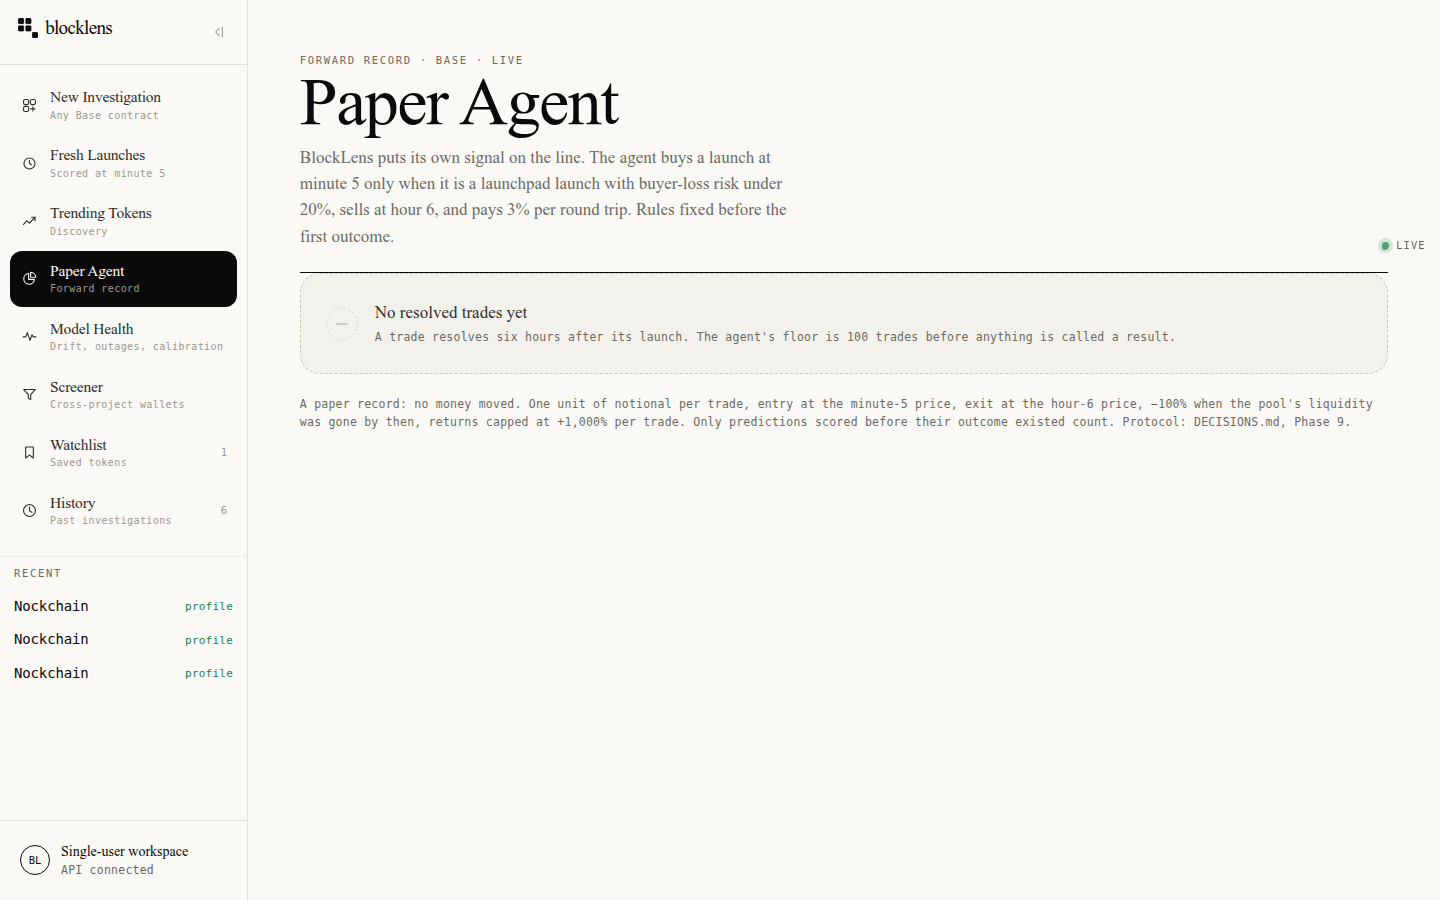
\includegraphics[width=\textwidth]{figures/portfolio.png}\caption{Paper Agent page (empty state on a fresh store; the live deployment shows the 850-trade book).}\end{figure}
\begin{figure}[H]\centering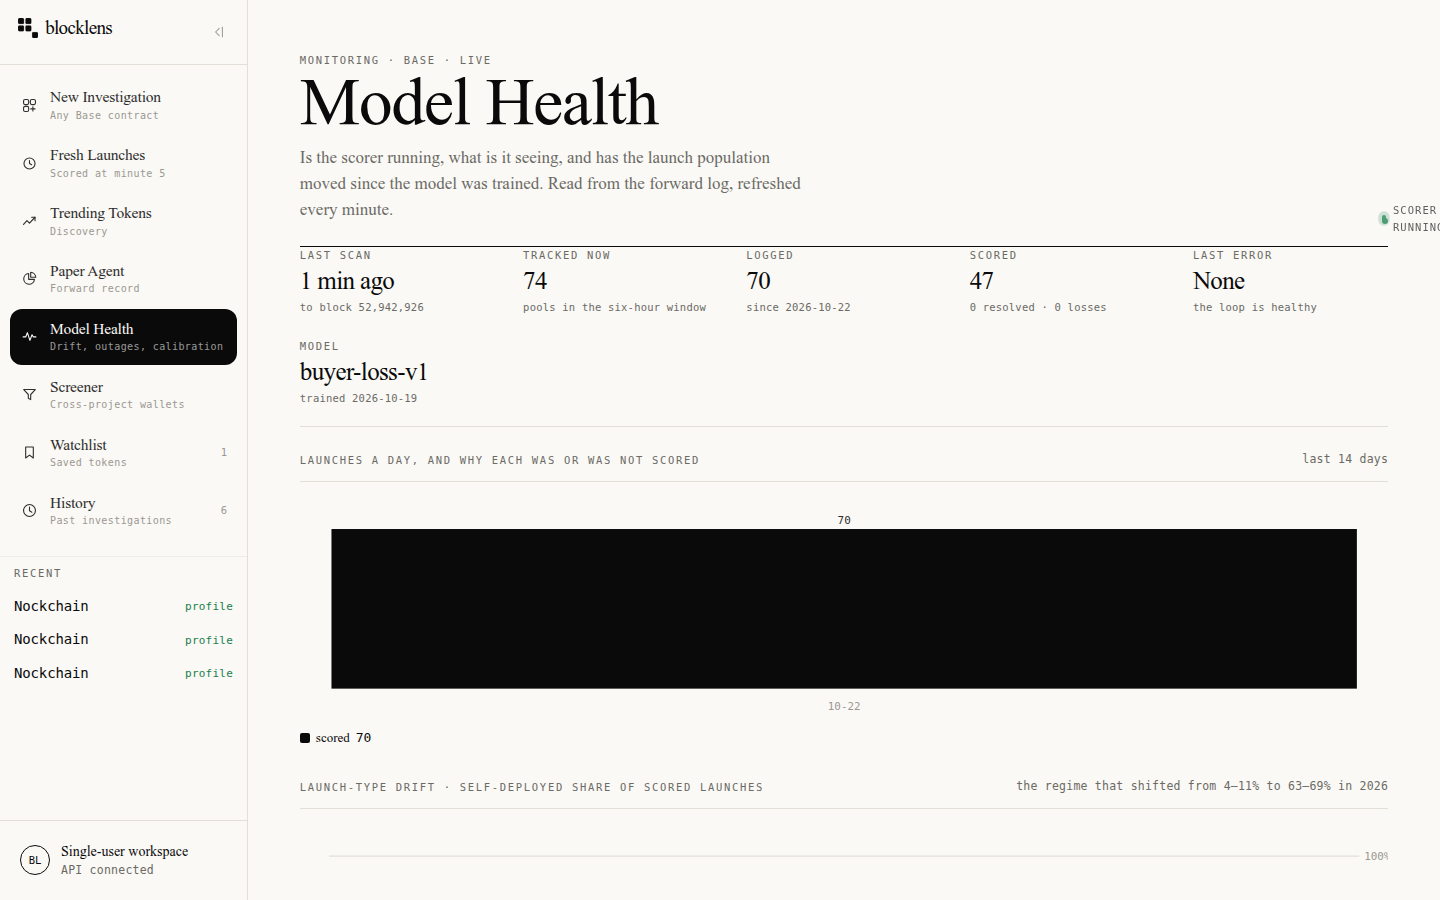
\includegraphics[width=\textwidth]{figures/model.png}\caption{Model Health page.}\end{figure}
\begin{figure}[H]\centering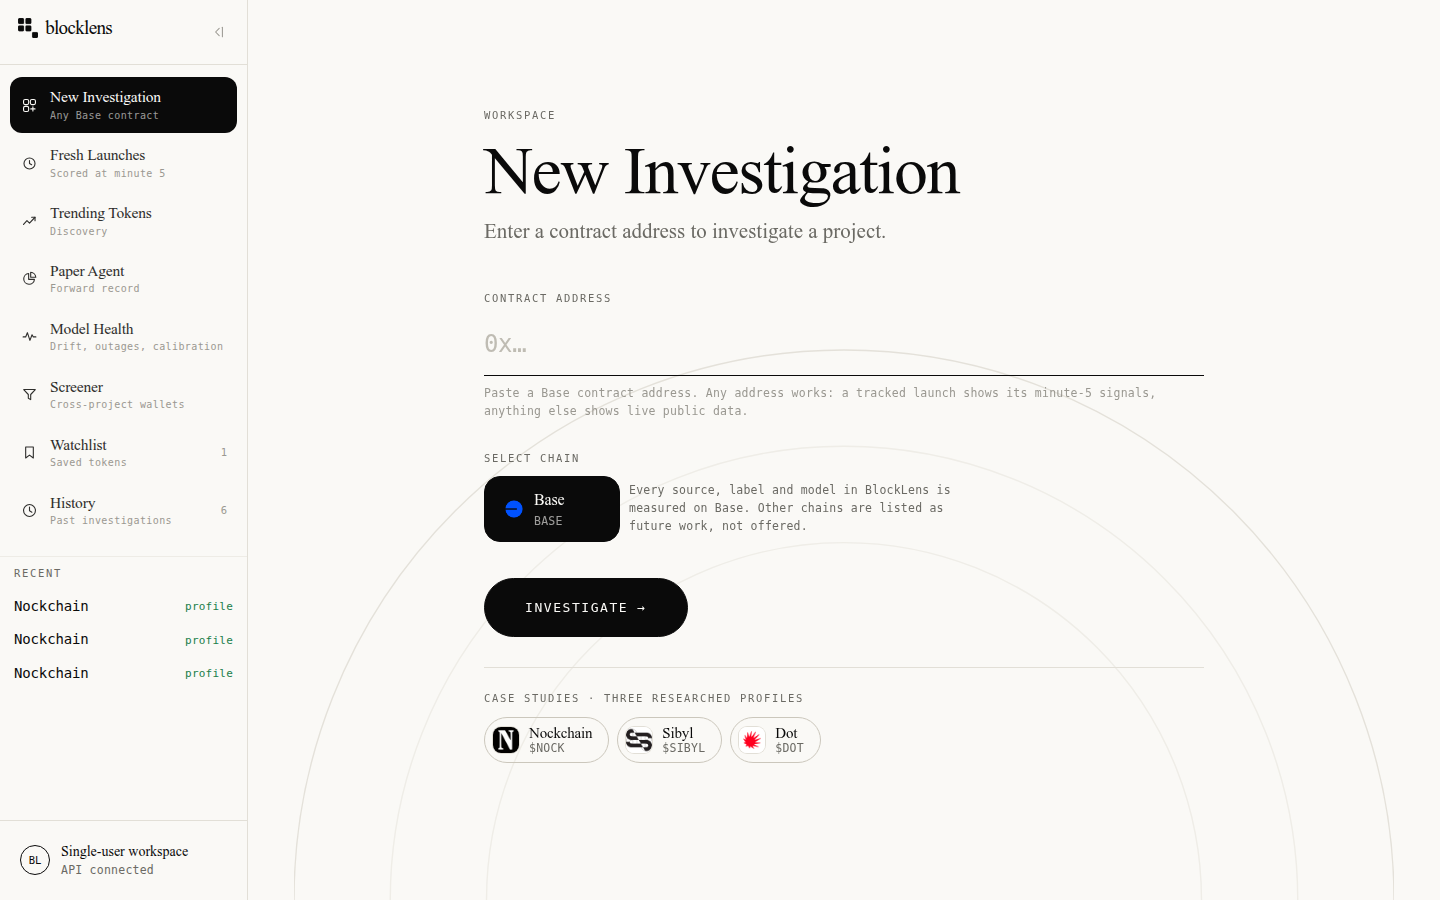
\includegraphics[width=\textwidth]{figures/new.png}\caption{New Investigation: any Base address; the three case studies offered as such.}\end{figure}
\begin{figure}[H]\centering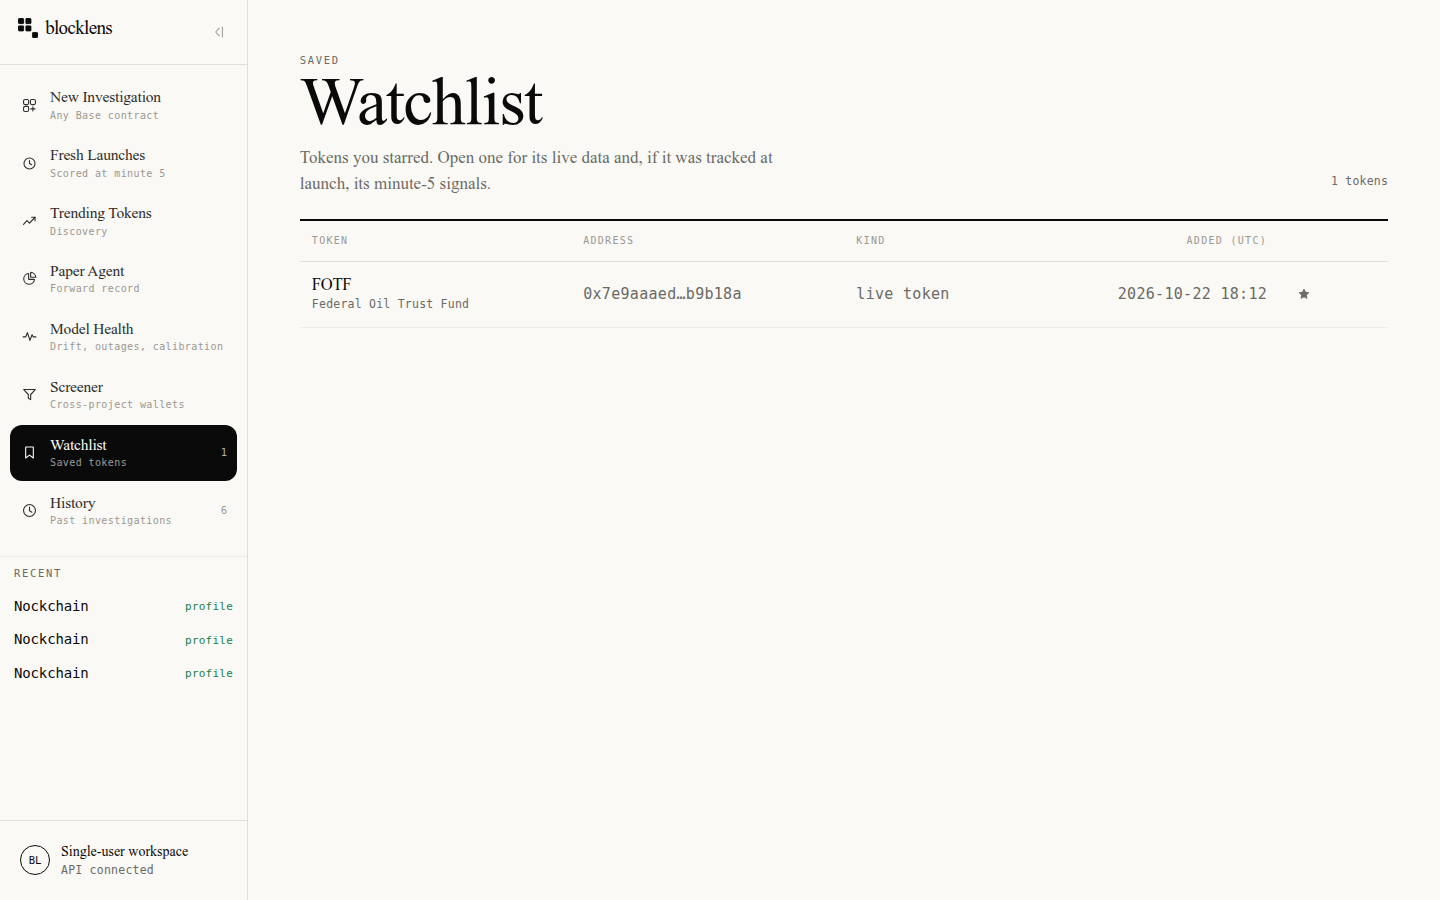
\includegraphics[width=\textwidth]{figures/watchlist.png}\caption{Watchlist held by the API.}\end{figure}
\todo{Add: a screenshot of the GitHub Actions run list and of one green pull request.}

\chapter{Additional Design Diagrams}
\begin{figure}[H]
\centering
\begin{adjustbox}{max width=\textwidth}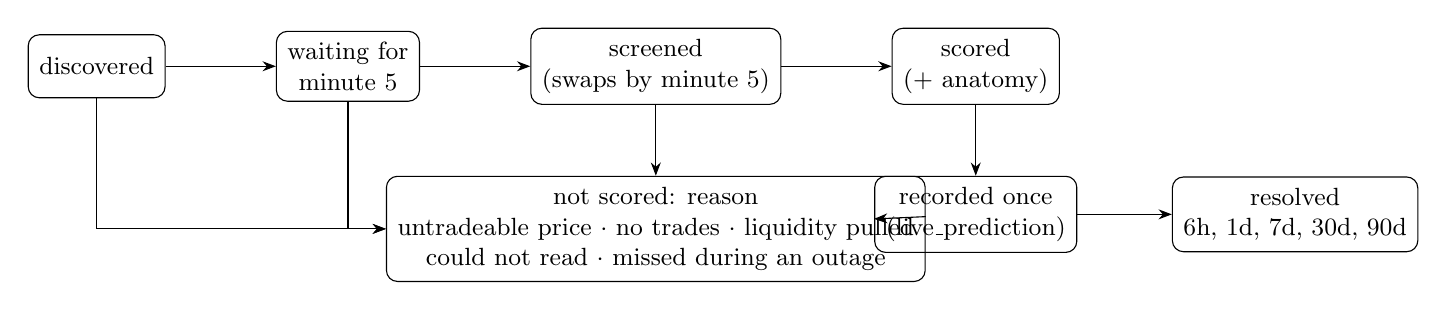
\begin{tikzpicture}[font=\small, >={Stealth}, st/.style={draw, rounded corners, align=center, inner sep=4pt, minimum height=0.8cm}]
  \node[st] (disc) at (0,0) {discovered};
  \node[st, right=1.4cm of disc] (wait) {waiting for\\minute 5};
  \node[st, right=1.4cm of wait] (scr) {screened\\(swaps by minute 5)};
  \node[st, right=1.4cm of scr] (scored) {scored\\(+ anatomy)};
  \node[st, below=0.9cm of scr] (not) {not scored: reason\\untradeable price $\cdot$ no trades $\cdot$ liquidity pulled\\could not read $\cdot$ missed during an outage};
  \node[st, below=0.9cm of scored] (rec) {recorded once\\(live\_prediction)};
  \node[st, right=1.2cm of rec] (res) {resolved\\6h, 1d, 7d, 30d, 90d};
  \draw[->] (disc) -- (wait); \draw[->] (wait) -- (scr); \draw[->] (scr) -- (scored);
  \draw[->] (disc) |- (not); \draw[->] (scr) -- (not); \draw[->] (wait) |- (not);
  \draw[->] (scored) -- (rec); \draw[->] (not) -- (rec); \draw[->] (rec) -- (res);
\end{tikzpicture}\end{adjustbox}
\caption{State diagram of a launch in the live scorer.}
\end{figure}
\begin{figure}[H]
\centering
\begin{adjustbox}{max width=\textwidth}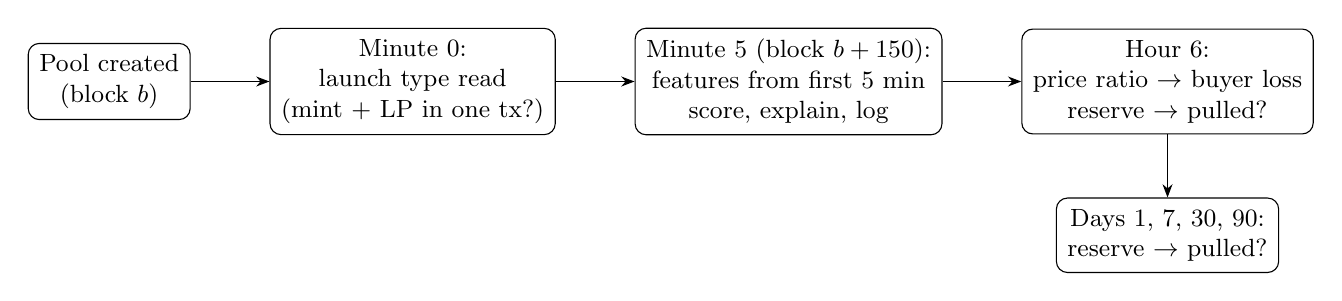
\begin{tikzpicture}[font=\small, >={Stealth}, st/.style={draw, rounded corners, align=center, inner sep=4pt}]
  \node[st] (a) at (0,0) {Pool created\\(block $b$)};
  \node[st, right=1cm of a] (b) {Minute 0:\\launch type read\\(mint + LP in one tx?)};
  \node[st, right=1cm of b] (c) {Minute 5 (block $b+150$):\\features from first 5 min\\score, explain, log};
  \node[st, right=1cm of c] (d) {Hour 6:\\price ratio $\to$ buyer loss\\reserve $\to$ pulled?};
  \node[st, below=0.8cm of d] (e) {Days 1, 7, 30, 90:\\reserve $\to$ pulled?};
  \draw[->] (a) -- (b); \draw[->] (b) -- (c); \draw[->] (c) -- (d); \draw[->] (d) -- (e);
\end{tikzpicture}\end{adjustbox}
\caption{Timeline of one launch from creation to resolution.}
\end{figure}
\begin{figure}[H]\centering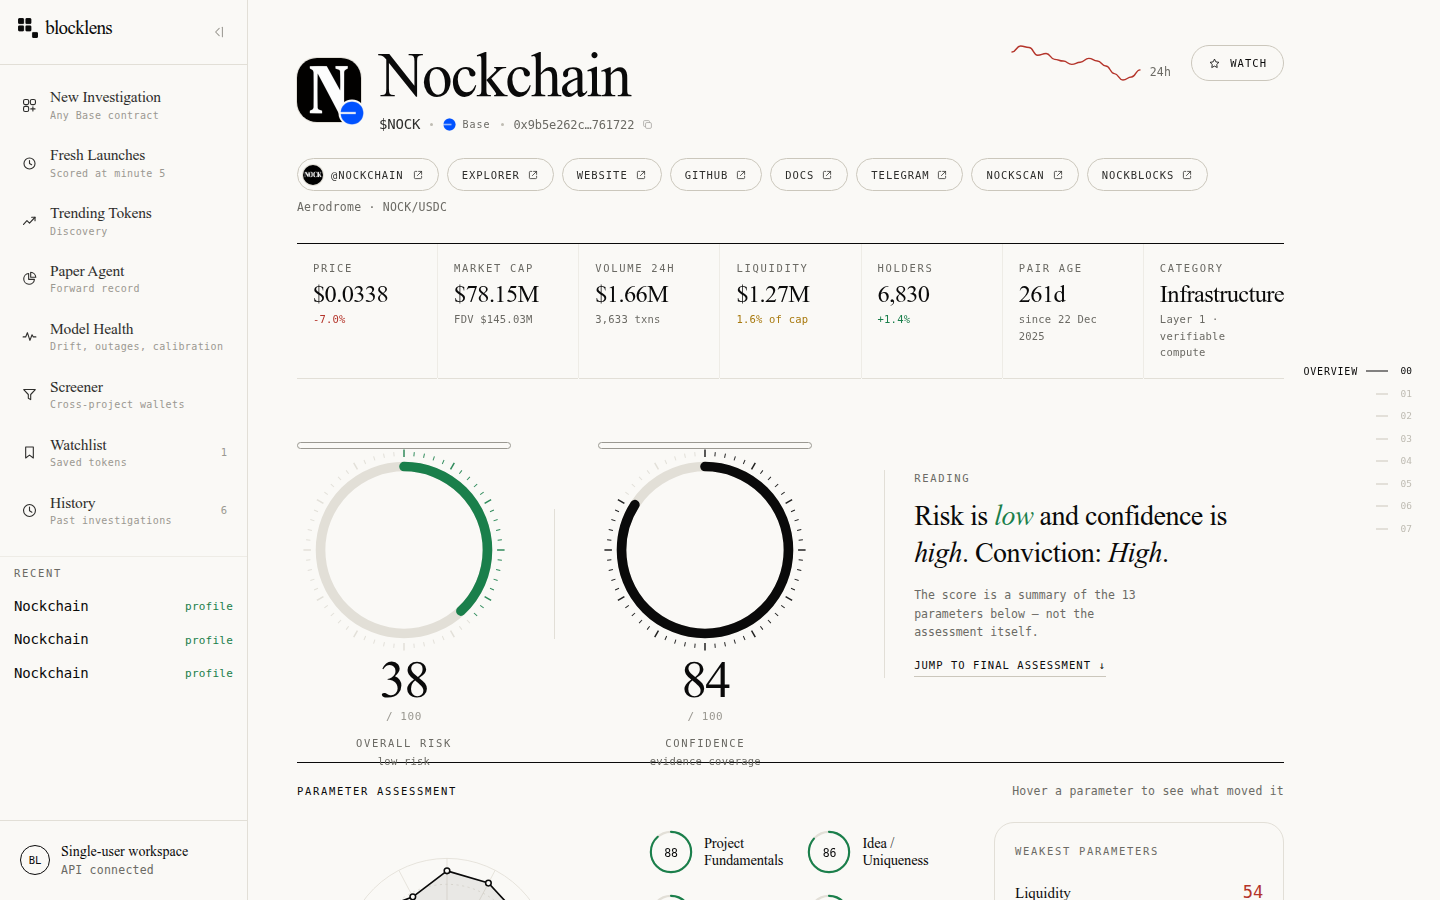
\includegraphics[width=\textwidth]{figures/profile.png}\caption{A case-study profile (Nockchain), eight sections, each marked Sourced or Sample.}\end{figure}
\begin{figure}[H]\centering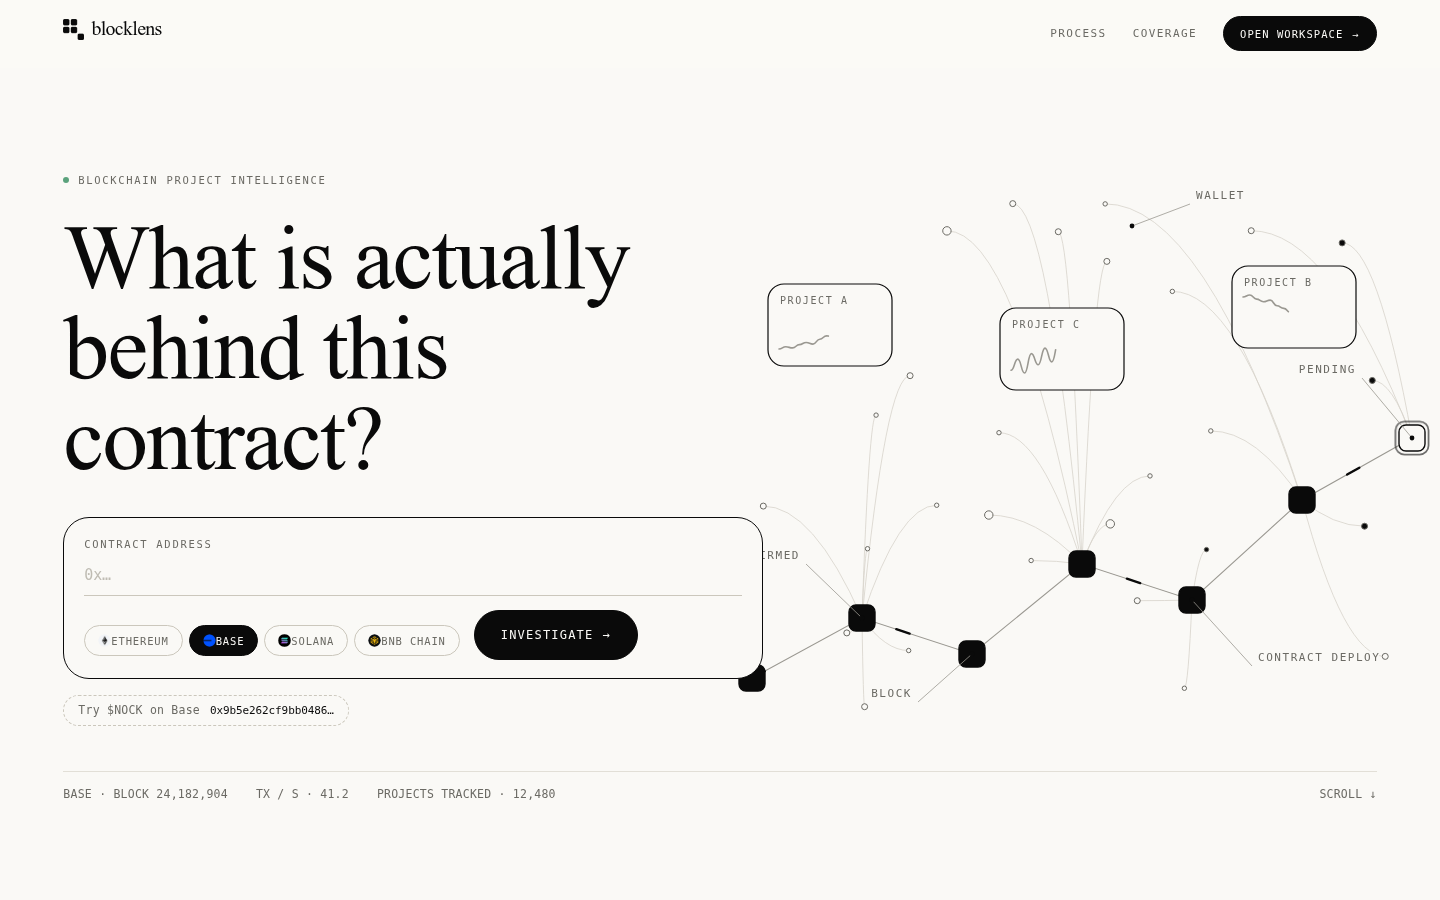
\includegraphics[width=\textwidth]{figures/landing.png}\caption{Landing page.}\end{figure}

\chapter{Meeting and Progress Evidence}
Supervisory meetings with Ms. Noshina Tariq were held twice a week. Attendees at each: Ms. Noshina Tariq, Abbas, Abdullah Bin Nasir, Shahmir Khan Lughmani. The agenda and decisions below are taken from the project's dated decision log and commit history for each week.

\begin{longtable}{p{0.12\textwidth}p{0.42\textwidth}p{0.4\textwidth}}
\toprule
Date & Discussed & Decisions / actions\\
\midrule
\endhead
02 Oct 2026 & Outcome of the proposal defence (approved with minor modifications); the seven comments; the rule that the project does only unpaid work & Address every comment with evidence; run feasibility spikes on the free sources before writing pipeline code; candidate chains Base, Solana, Robinhood Chain\\
06 Oct 2026 & Design of the spikes: which endpoints, which limits to measure, how to record them & Measure \code{eth_getLogs} caps, archive depth, DexScreener feeds and rate limits; record everything in \code{spikes/FINDINGS.md}\\
09 Oct 2026 & Early spike results: 1,000-block log cap, DexScreener feeds carry no Base tokens, Uniswap V4 is most of the chain & Discovery from chain events; a write gate with \code{as_of_ts}; Base chosen on measured grounds\\
13 Oct 2026 & Phase 1 acceptance (159 windows, zero cost); the label definition and its thresholds; the V4 reserve problem & Sample reserves at blocks instead of reconstructing; token-side reserve for V4; sweep every threshold\\
16 Oct 2026 & Phase 3 graph and the first model's AUC 0.97; the supervisor's and team's concern that the result was too good; the committee's CI/CD requirement & Run a leakage and censoring audit before any number is reported; plan the CI/CD pipeline and branch process\\
20 Oct 2026 & Audit outcome (Phase 4 withdrawn), the redesigned sample and the two signals; the live feed demo; the forward test and paper agent protocols; narrowing the scope & Pre-register the forward test; cut KOL, simulated portfolio and unmeasured chains; write the scope document; start the report\\
\bottomrule
\end{longtable}


\bibliographystyle{IEEEtranN}
\bibliography{references/references}
\end{document}
